\documentclass{beamer}
%\documentclass[handout]{beamer}
\usetheme{Marburg}
\useoutertheme{infolines}
\newcommand{\answers}{1}

\usepackage{amsmath}
\usepackage{caption}
\usepackage{color}
\usepackage{enumerate}
\usepackage{listings}
\usepackage{hyperref}
\usepackage{mathrsfs}
\usepackage{natbib}
\usepackage{url}

\providecommand{\all}{\ \forall \ }
\providecommand{\bs}{\backslash}
\providecommand{\e}{\varepsilon}
\providecommand{\E}{\ \exists \ }
\providecommand{\lm}[2]{\lim_{#1 \rightarrow #2}}
\providecommand{\m}[1]{\mathbb{#1}}
\providecommand{\nv}{{}^{-1}}
\providecommand{\ov}[1]{\overline{#1}}
\providecommand{\p}{\newpage}
\providecommand{\q}{$\quad$ \newline}
\providecommand{\rt}{\rightarrow}
\providecommand{\Rt}{\Rightarrow}
\providecommand{\vc}[1]{\boldsymbol{#1}}
\providecommand{\wh}[1]{\widehat{#1}}

\hypersetup{colorlinks,linkcolor=,urlcolor=blue}
\numberwithin{equation}{section}

\definecolor{dkgreen}{rgb}{0,0.6,0}
\definecolor{gray}{rgb}{0.5,0.5,0.5}
\definecolor{mauve}{rgb}{0.58,0,0.82}

\lstset{ 
  language=C,                % the language of the code
  basicstyle= \footnotesize,           % the size of the fonts that are used for the code
  numbers=left,
  numberfirstline=true,
  numbersep=5pt,                  % how far the line-numbers are from the code
  backgroundcolor=\color{white},      % choose the background color. You must add \usepackage{color}
  showspaces=false,               % show spaces adding particular underscores
  showstringspaces=false,         % underline spaces within strings
  showtabs=false,                 % show tabs within strings adding particular underscores
  frame=lrb,                   % adds a frame around the code
  rulecolor=\color{black},        % if not set, the frame-color may be changed on line-breaks within not-black text 
  tabsize=2,                      % sets default tabsize to 2 spaces
  captionpos=t,                   % sets the caption-position 
  breaklines=true,                % sets automatic line breaking
  breakatwhitespace=false,        % sets if automatic breaks should only happen at whitespace
  %title=\lstname,                   % show the filename of files included with \lstinputlisting;
  keywordstyle=\color{blue},          % keyword style
  commentstyle=\color{gray},       % comment style
  stringstyle=\color{dkgreen},         % string literal style
  escapeinside={\%*}{*)},            % if you want to add LaTeX within your code
  morekeywords={*, ...},               % if you want to add more keywords to the set
  xleftmargin=0.2in, % left horizontal offset of caption box
  xrightmargin=-.03in % right horizontal offset of caption box
}

%\DeclareCaptionFont{white}{\color{white}}
%\DeclareCaptionFormat{listing}{\parbox{\textwidth}{\colorbox{gray}{\parbox{\textwidth}{#1#2#3}}\vskip-0.05in}}
%\captionsetup[lstlisting]{format = listing, labelfont = white, textfont = white}
%For caption-free listings, comment out the 3 lines above and uncomment the 2 lines below.
 \captionsetup{labelformat = empty, labelsep = none}
 \lstset{frame = single}

\title{CUDA C: performance measurement and memory}
\author{Will Landau}
\date{October 14, 2013}
\institute{Iowa State University}

\begin{document}

\begin{frame}
\titlepage
 \end{frame}
 
 \begin{frame}
\frametitle{Outline}
\tableofcontents
\end{frame}
 
 \AtBeginSection[]
{
   \begin{frame}
       \frametitle{Outline}
       \tableofcontents[currentsection]
   \end{frame}
}

\section{Timing kernels on the GPU}


\begin{frame}[fragile]
\frametitle{Measuring CPU time}
\begin{lstlisting}
#include <stdio.h>
#include <time.h>

int main(){
  float elapsedTime;
  clock_t start = clock();
  
  // SOME CPU CODE YOU WANT TO TIME
  
  elapsedTime = ((double) clock() - start) / CLOCKS_PER_SEC;
  
  pritnf("CPU time elapsed: %f seconds \n", elapsedTime);
  return 0;
}
\end{lstlisting}
\end{frame}


\begin{frame}[fragile]
\frametitle{Events}

\begin{itemize}
\item {\bf Event}: a time stamp on the GPU
\pause \item Use events to measure GPU execution time.
\pause \item {\tt time.cu}:
\end{itemize}

\lstset{basicstyle=\tiny}
\begin{lstlisting}
#include <stdlib.h>
#include <stdio.h>
#include <cuda.h>
#include <cuda_runtime.h>

int main(){
  float   elapsedTime;
  cudaEvent_t start, stop;
  cudaEventCreate(&start);
  cudaEventCreate(&stop);
  cudaEventRecord( start, 0 );

  // SOME GPU WORK YOU WANT TIMED HERE

  cudaEventRecord( stop, 0 );
  cudaEventSynchronize( stop );
  cudaEventElapsedTime( &elapsedTime, start, stop );
  cudaEventDestroy( start );
  cudaEventDestroy( stop );
  printf("GPU Time elapsed: %f milliseconds\n", elapsedTime);
}
\end{lstlisting}

\begin{itemize}
\pause \item GPU time and CPU time must be measured separately.
\end{itemize}
\end{frame}


\begin{frame}[fragile]
\frametitle{Example: {\tt pairwise\_sum\_timed.cu}} \lstset{basicstyle=\tiny}
\begin{lstlisting}[name=pstime]
#include <stdio.h> 
#include <stdlib.h> 
#include <math.h>
#include <time.h>
#include <unistd.h>
#include <cuda.h>
#include <cuda_runtime.h> 

/* This program computes the sum of the elements of 
 * vector v using the pairwise (cascading) sum algorithm. */

#define N 1024 // length of vector v. MUST BE A POWER OF 2!!!

// Fill the vector v with n random floating point numbers.
void vfill(float* v, int n){
  int i;
  for(i = 0; i < n; i++){
    v[i] = (float) rand() / RAND_MAX;
  }
}

// Print the vector v.
void vprint(float* v, int n){
  int i;
  printf("v = \n");
  for(i = 0; i < n; i++){
    printf("%7.3f\n", v[i]);
  }
  printf("\n");
}
\end{lstlisting}
\end{frame}

\begin{frame}[fragile]
\frametitle{Example: {\tt pairwise\_sum\_timed.cu}} \lstset{basicstyle=\tiny}
\begin{lstlisting}[name=pstime]
// Pairwise-sum the elements of vector v and store the result in v[0]. 
__global__ void psum(float *v){ 
  int t = threadIdx.x; // Thread index.
  int n = blockDim.x; // Should be half the length of v.

  while (n != 0) {
    if(t < n)
      v[t] += v[t + n];  
    __syncthreads();    
    n /= 2; 
  }
}

// Linear sum the elements of vector v and return the result
float lsum(float *v, int len){
  float s = 0;
  int i;
  for(i = 0; i < len; i++){
    s += v[i];
  }
  return s;
}

\end{lstlisting}
\end{frame}

\begin{frame}[fragile]
\frametitle{Example: {\tt pairwise\_sum\_timed.cu}} \lstset{basicstyle=\tiny}
\begin{lstlisting}[name=pstime]
int main (void){ 
  float *v_h, *v_d; // host and device copies of our vector, respectively
  
  // dynamically allocate memory on the host for v_h
  v_h = (float*) malloc(N * sizeof(*v_h)); 
  
  // dynamically allocate memory on the device for v_d
  cudaMalloc ((float**) &v_d, N *sizeof(*v_d)); 
  
  // Fill v_h with N random floating point numbers.
  vfill(v_h, N);

  // Print v_h to the console
  // vprint(v_h, N);
  
  // Write the contents of v_h to v_d
  cudaMemcpy( v_d, v_h, N * sizeof(float), cudaMemcpyHostToDevice );
    
  // compute the linear sum of the elements of v_h on the CPU and return the result
  // also, time the result.
  clock_t start = clock();
  float s = lsum(v_h, N);
\end{lstlisting}
\end{frame}


\begin{frame}[fragile]
\frametitle{Example: {\tt pairwise\_sum\_timed.cu}} \lstset{basicstyle=\tiny}
\begin{lstlisting}[name=pstime]
  float elapsedTime = ((float) clock() - start) / CLOCKS_PER_SEC;
  printf("Linear Sum = %7.3f, CPU Time elapsed: %f seconds\n", s, elapsedTime);
 
  // Compute the pairwise sum of the elements of v_d and store the result in v_d[0].
  // Also, time the computation.
  
  float   gpuElapsedTime;
  cudaEvent_t gpuStart, gpuStop;
  cudaEventCreate(&gpuStart);
  cudaEventCreate(&gpuStop);
  cudaEventRecord( gpuStart, 0 );

 psum<<< 1, N/2 >>>(v_d);
  
  cudaEventRecord( gpuStop, 0 );
  cudaEventSynchronize( gpuStop );
  cudaEventElapsedTime( &gpuElapsedTime, gpuStart, gpuStop ); // time in milliseconds
  cudaEventDestroy( gpuStart );
  cudaEventDestroy( gpuStop );
  
  // Write the pairwise sum, v_d[0], to v_h[0].
  cudaMemcpy(v_h, v_d, sizeof(float), cudaMemcpyDeviceToHost );
\end{lstlisting}
\end{frame}


\begin{frame}[fragile]
\frametitle{Example: {\tt pairwise\_sum\_timed.cu}} \lstset{basicstyle=\tiny}
\begin{lstlisting}[name=pstime]
  // Print the pairwise sum.
  printf("Pairwise Sum = %7.3f, GPU Time elapsed: %f seconds\n", v_h[0], gpuElapsedTime/1000.0);
   
  // Free dynamically-allocated host memory
  free(v_h);

  // Free dynamically-allocated device memory    
  cudaFree(&v_d);
}
\end{lstlisting}

\lstset{basicstyle=\tiny}

\begin{itemize}
\pause \item Output:
\end{itemize}
\begin{lstlisting}
> nvcc pairwise_sum_timed.cu -o pairwise_sum_timed
> ./pairwise_sum_timed
Linear Sum = 518.913, CPU Time elapsed: 0.000000 seconds
Pairwise Sum = 518.913, GPU Time elapsed: 0.000037 seconds
\end{lstlisting}
\end{frame}



\section{Memory}

\begin{frame}
\frametitle{Types of memory}
\begin{center}
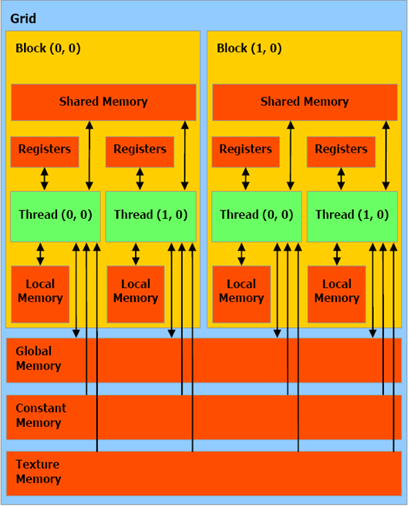
\includegraphics[scale=0.42]{../../fig/memory.png}
\end{center}
\end{frame}



\begin{frame}[fragile]
\frametitle{What happens in {\tt myKernel<<<2, 2>>>(b, t)}?}
\begin{lstlisting}
__global__ void myKernel(int *b_global, int *t_global){

  __shared__ int t;
  __shared__ int b;

  int b_local, t_local;
  
  *t_global = threadIdx.x;
  *b_global = blockIdx.x;
  
   t_shared = threadIdx.x;
   b_shared = blockIdx.x;
  
   t_local = threadIdx.x;
   b_local = blockIdx.x;
}
\end{lstlisting}
\end{frame}


\begin{frame}<handout:\answers>
\frametitle{At the end of {\tt myKernel<<<4, 7>>>(b, t)}...} \small
\begin{itemize}
\item {\tt b\_local} and {\tt t\_local} are in local memory (or registers), so each thread gets a copy.

\pause \begin{center}
\begin{tabular}{c|cccc}
(block, thread) & (0, 0) & (0, 1) & (1, 0) & (1, 1) \\ \hline
{\tt b\_local} & 0 & 0 & 1 & 1 \\ \hline
{\tt t\_local} & 0 & 1 & 0 & 1
\end{tabular}
\end{center}


\pause \item {\tt b\_shared} and {\tt t\_shared} are in shared memory, so each block gets a copy.

\pause \begin{center}
\begin{tabular}{c|cccc}
(block, thread) & (0, 0) & (0, 1) & (1, 0) & (1, 1) \\ \hline
{\tt b\_shared} & 0 & 0 & 1 & 1 \\ \hline
{\tt t\_shared} & ? & ? & ? & ?
\end{tabular}
\end{center}

\begin{itemize}
\pause \item ? = last thread in its block to write to {\tt t\_shared}.
\end{itemize}
\end{itemize}
\end{frame}


\begin{frame}<handout:\answers>
\frametitle{At the end of {\tt myKernel<<<4, 7>>>(b, t)}...} \small
\begin{itemize}
\item {\tt b\_global} and {\tt t\_global} point to global memory, so there is only one copy.

\pause \begin{center}
\begin{tabular}{c|cccc}
(block, thread) & (0, 0) & (0, 1) & (1, 0) & (1, 1) \\ \hline
{\tt *b\_global} & ?? & ?? & ?? & ?? \\ \hline
{\tt *t\_global} & ? & ? & ? & ?
\end{tabular}
\end{center}

\begin{itemize}
\pause \item  ? = last thread in its block to write to {\tt *t\_global}.
\pause \item ?? = block of the last thread to write to {\tt *b\_global}.
\end{itemize}
\end{itemize}
\end{frame}


\begin{frame}
\frametitle{Example: dot product}

\begin{align*}
\vc{a} \bullet \vc{b} = (a_0, \ldots, a_{15}) \bullet (b_0, \ldots, b_{15})  = a_0 \cdot b_0 + \cdots + a_{15} \cdot b_{15}
\end{align*}

\begin{enumerate}
\pause \item In this example, spawn 2 blocks and 4 threads per block.
\pause \item Give each block a subvector of ${\vc a}$ and an analogous subvector of ${\vc b}$.
\begin{itemize}
\pause \item Block 0:
\begin{align*}
&(a_0, a_1, a_2, a_3, \ a_8, a_9, a_{10}, a_{11}) \\
&(b_0, b_1, b_2, b_3, \ b_8, b_9, b_{10}, b_{11}) 
\end{align*}
\pause \item Block 1:
\begin{align*}
&(a_4, a_5, a_6, a_7, \ a_{12}, a_{13}, a_{14}, a_{15}) \\
&(b_4, b_5, b_6, b_7, \ b_{12}, b_{13}, b_{14}, b_{15}) 
\end{align*}
\end{itemize}
\end{enumerate}
\end{frame}

\begin{frame}
\frametitle{Example: dot product}


\begin{enumerate} \setcounter{enumi}{2}
\item Create an array, {\tt cache}, in shared memory:

\begin{itemize}
\pause \item Block 0:
\begin{align*}
\text{cache[0]} &= a_0 \cdot b_0 + a_8 \cdot b_8 \\
\text{cache[1]} &= a_1 \cdot b_1 + a_9 \cdot b_9 \\
\text{cache[2]} &= a_2 \cdot b_2 + a_{10} \cdot b_{10} \\
\text{cache[3]} &= a_3 \cdot b_3 + a_{11} \cdot b_{11} \\
\end{align*}
\pause \item Block 1:
\begin{align*}
\text{cache[0]} &= a_4 \cdot b_4 + a_{12} \cdot b_{12} \\
\text{cache[1]} &= a_5 \cdot b_5 + a_{13} \cdot b_{13} \\
\text{cache[2]} &= a_6 \cdot b_6 + a_{14} \cdot b_{14} \\
\text{cache[3]} &= a_7 \cdot b_7 + a_{15} \cdot b_{15} \\
\end{align*}
\end{itemize}
\end{enumerate}
\end{frame}




\begin{frame}
\frametitle{Example: dot product}

\begin{enumerate} \setcounter{enumi}{3}
\item Compute the pairwise sum of {\tt cache} in each block and write it to {\tt cache[0]}
\begin{itemize}
 \item Block 0:
\begin{align*}
\text{cache[0]} &= a_0 \cdot b_0 + a_8 \cdot b_8 \\
 &+ a_1 \cdot b_1 + a_9 \cdot b_9 \\
 &+ a_2 \cdot b_2 + a_{10} \cdot b_{10} \\
 &+ a_3 \cdot b_3 + a_{11} \cdot b_{11} \\
\end{align*}
\item Block 1:
\begin{align*}
\text{cache[0]} &= a_4 \cdot b_4 + a_{12} \cdot b_{12} \\
  &+ a_5 \cdot b_5 + a_{13} \cdot b_{13} \\
  &+ a_6 \cdot b_6 + a_{14} \cdot b_{14} \\
  &+ a_7 \cdot b_7 + a_{15} \cdot b_{15} \\
\end{align*}
\end{itemize}
\end{enumerate}
\end{frame}

\begin{frame}
\frametitle{Example: dot product}
\begin{enumerate} \setcounter{enumi}{4}
\item Compute an array, {\tt partial\_c} in global memory:
\begin{align*}
\text{partial\_c[0]} &= \text{cache[0] from block 0} \\
\text{partial\_c[1]} &= \text{cache[0] from block 1} \\
\end{align*}
\pause \item The pairwise sum of {\tt partial\_c} is the final answer.
\end{enumerate}
\end{frame}

\begin{frame}[fragile]
\frametitle{{\tt dot\_product.cu}} \lstset{basicstyle=\tiny}
\begin{lstlisting}[name=dp]
#include "../common/book.h" 
#include <stdio.h>
#include <stdlib.h>
#define imin(a,b) (a<b?a:b)

const int N = 32 * 1024;
const int threadsPerBlock = 256; 
const int blocksPerGrid = imin( 32, (N+threadsPerBlock-1) / threadsPerBlock );

__global__ void dot( float *a, float *b, float *partial_c ) { 

  __shared__ float cache[threadsPerBlock];
  int tid = threadIdx.x + blockIdx.x * blockDim.x; 
  int cacheIndex = threadIdx.x;
  float temp = 0; 

  while (tid < N) {
    temp += a[tid] * b[tid];
    tid += blockDim.x * gridDim.x;
  }

  // set the cache values
  cache[cacheIndex] = temp;
\end{lstlisting}
\end{frame}



\begin{frame}
\frametitle{{\tt dot<<<2, 4>>>(a, b, c)} with $N = 16$} 
\begin{center}
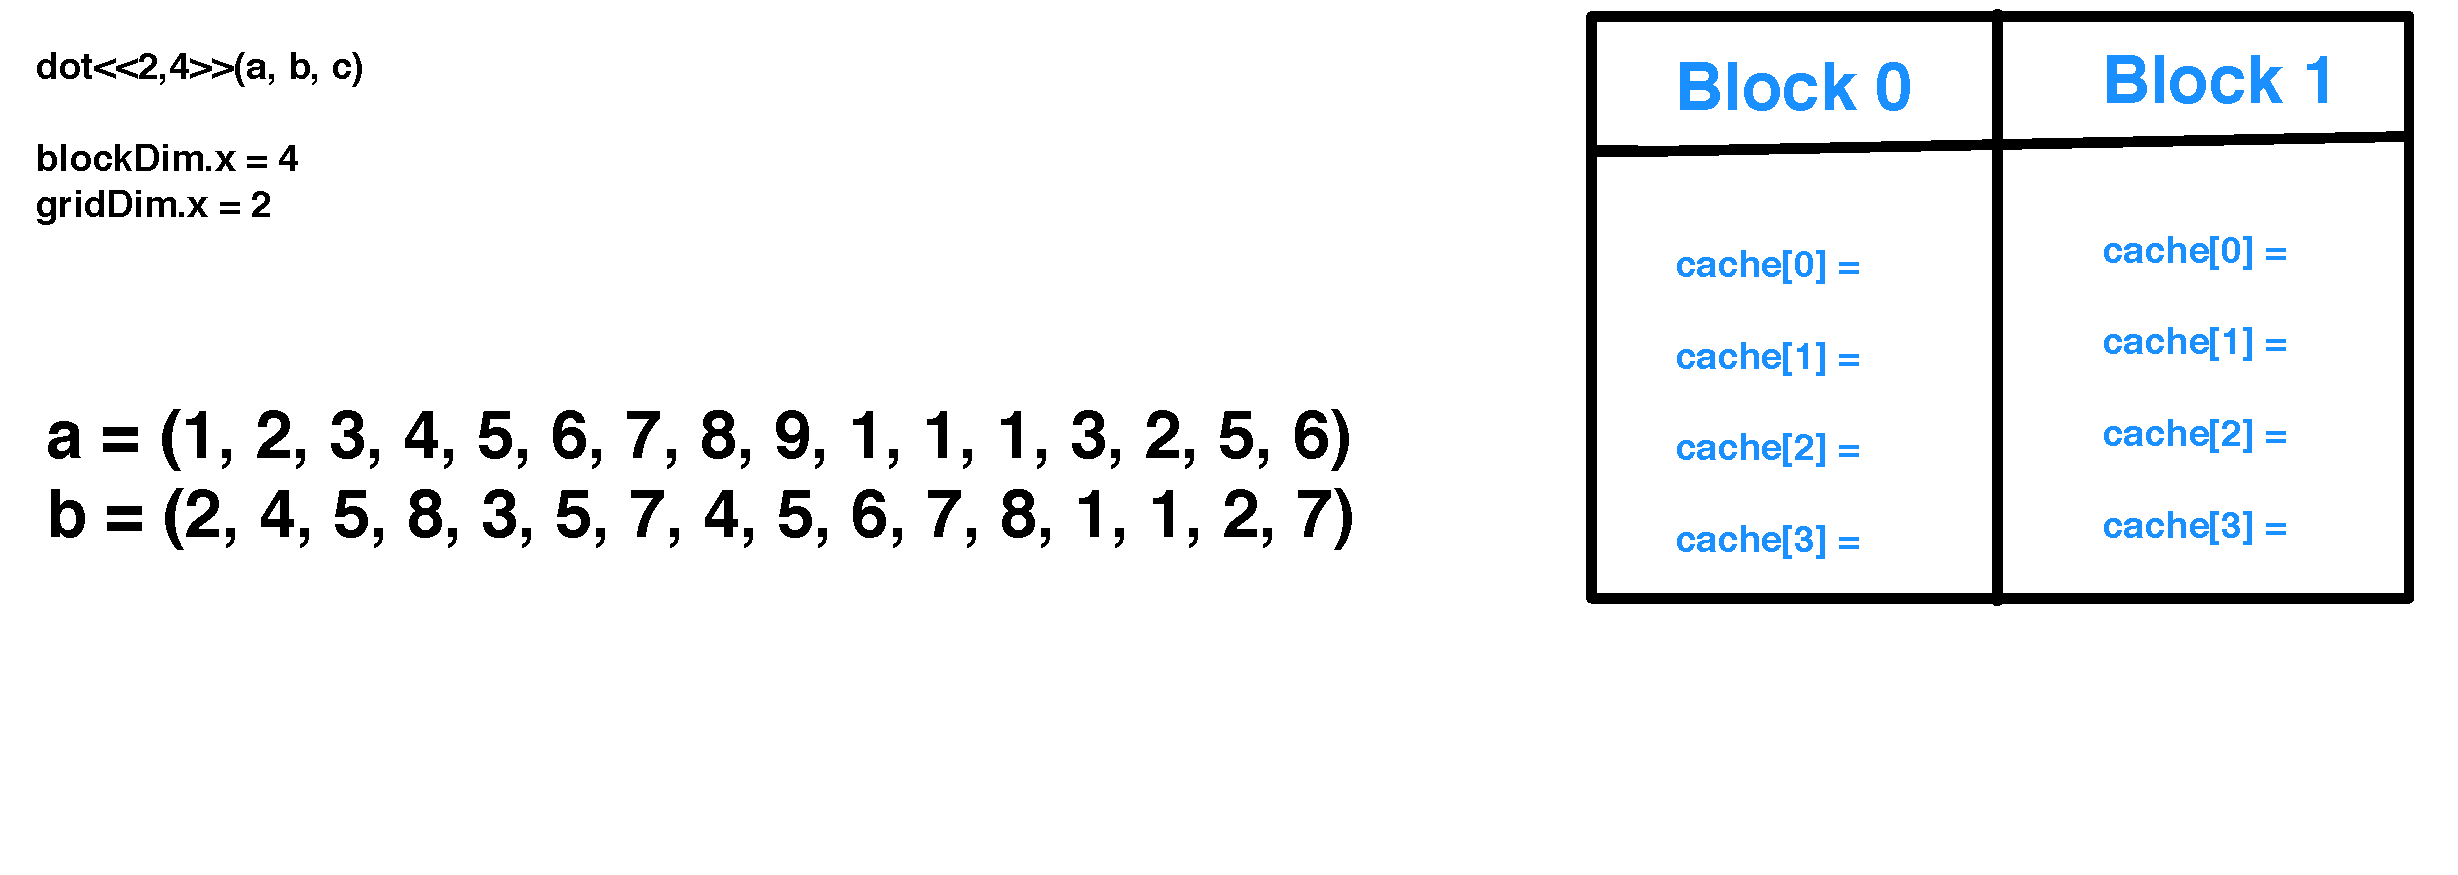
\includegraphics[scale=.23]{../../fig/dotconcept1}
\end{center}
\end{frame}
 
\begin{frame}
\frametitle{{\tt dot<<<2, 4>>>(a, b, c)} with $N = 16$}
\begin{center}
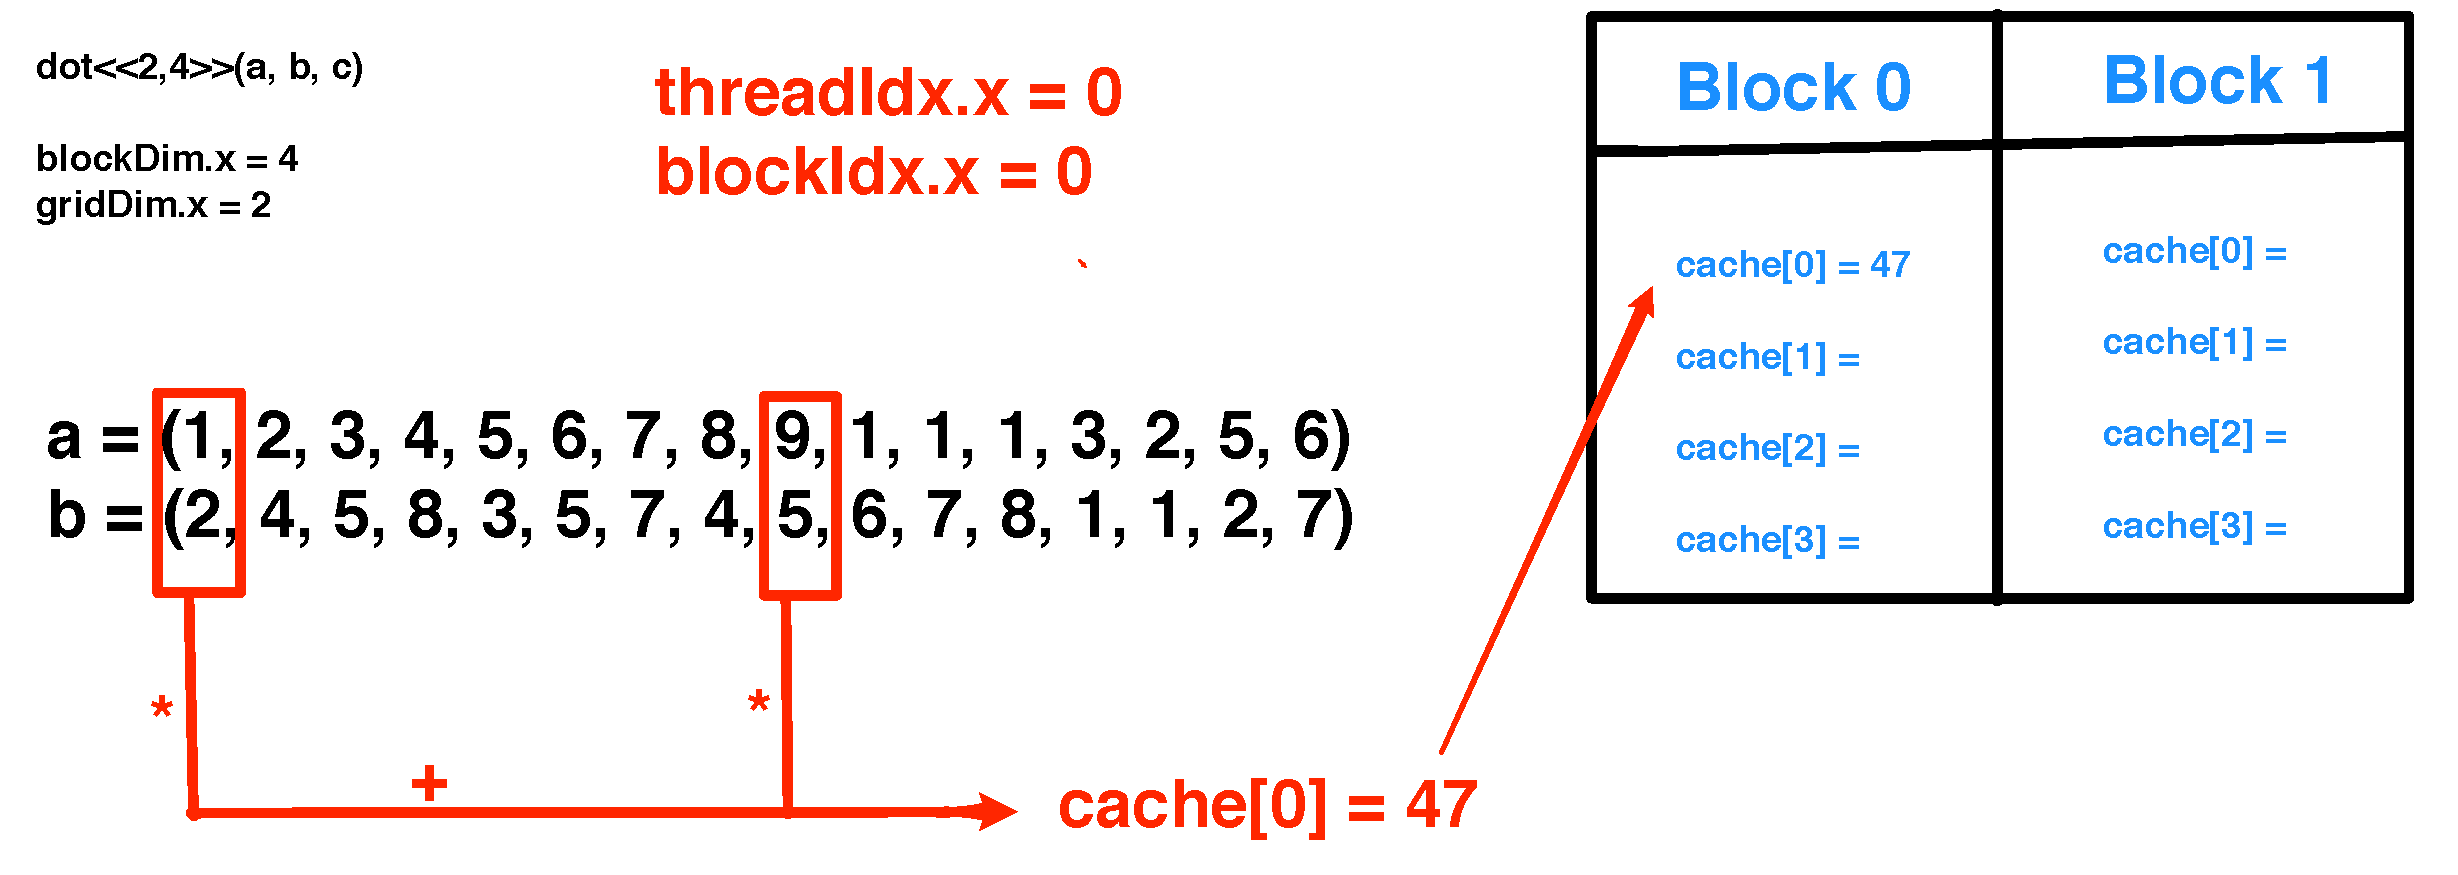
\includegraphics[scale=.23]{../../fig/dotconcept2}
\end{center}
\end{frame}
 
 \begin{frame}
\frametitle{{\tt dot<<<2, 4>>>(a, b, c)} with $N = 16$}
\begin{center}
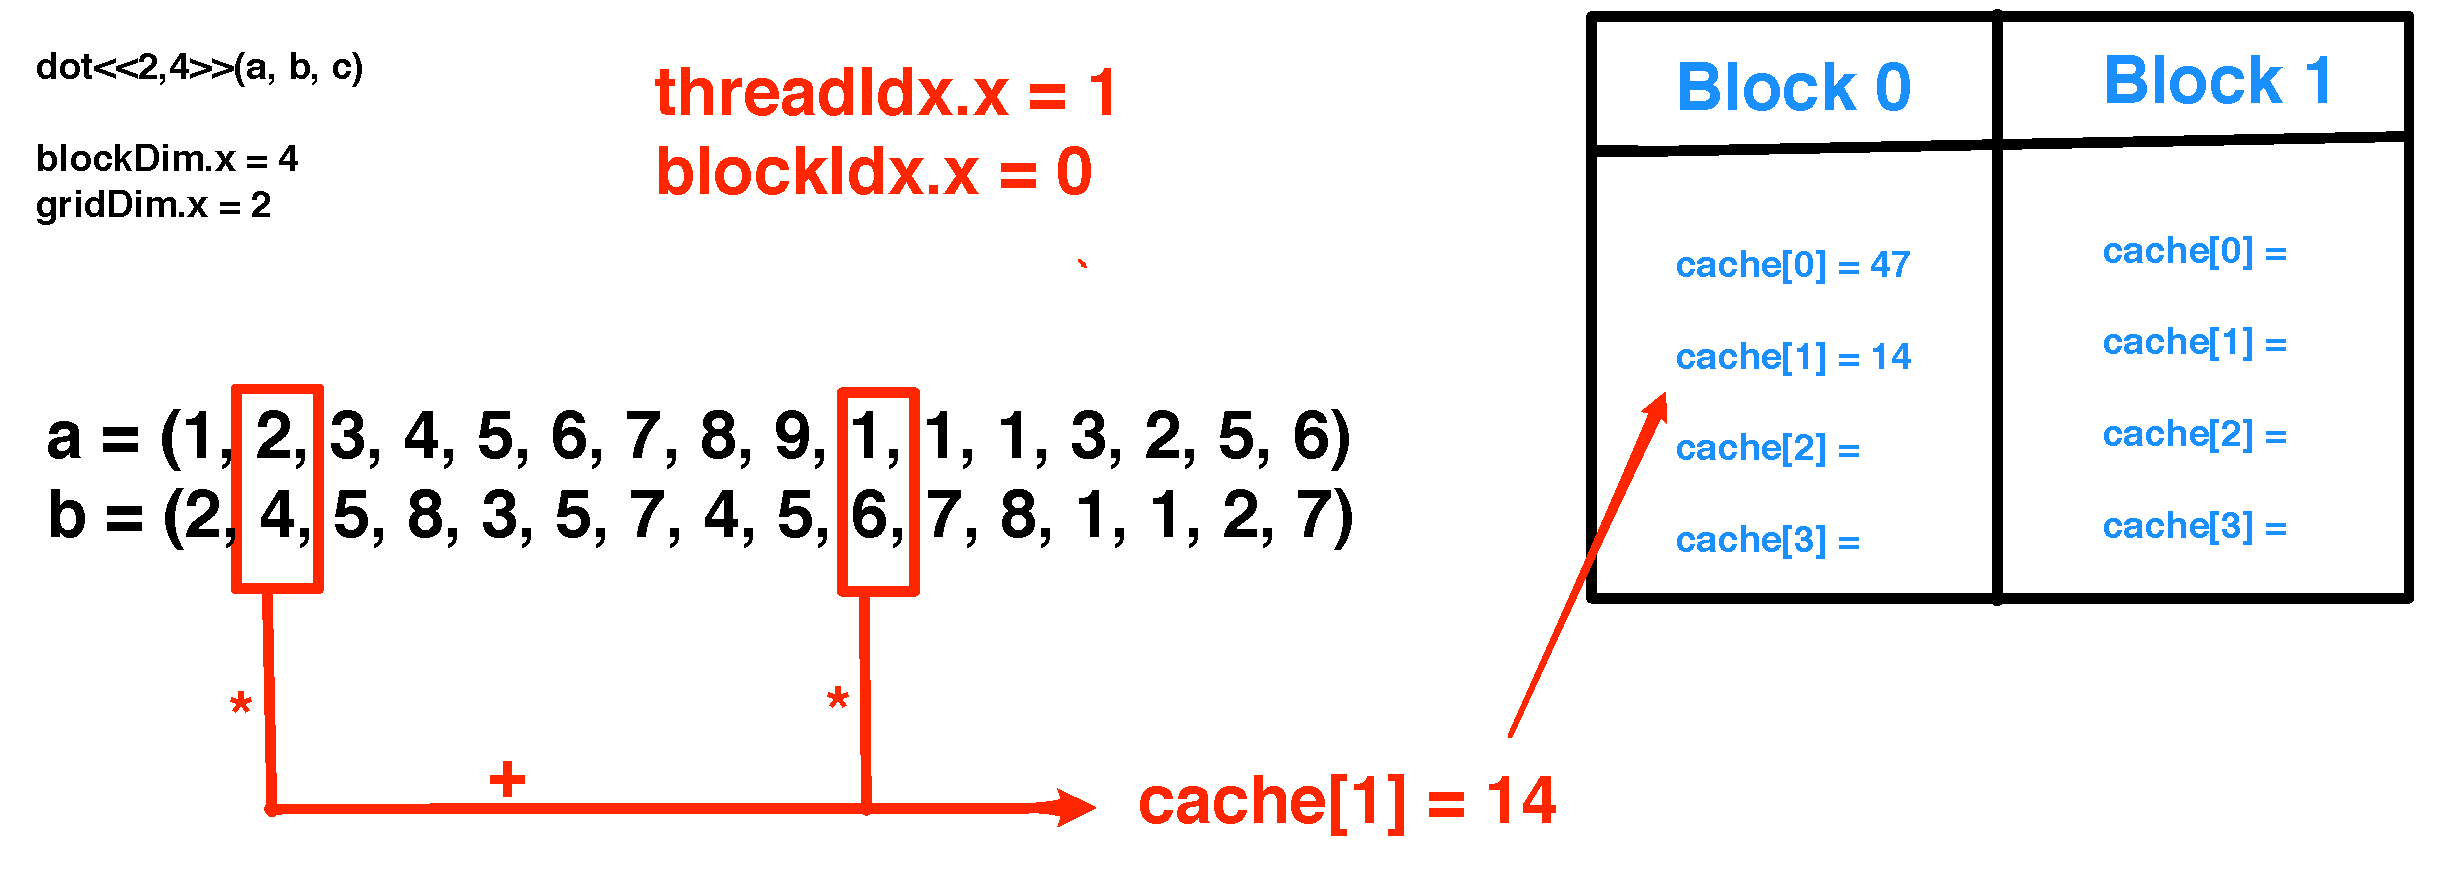
\includegraphics[scale=.23]{../../fig/dotconcept3}
\end{center}
\end{frame}
 
 \begin{frame}
\frametitle{{\tt dot<<<2, 4>>>(a, b, c)} with $N = 16$}
\begin{center}
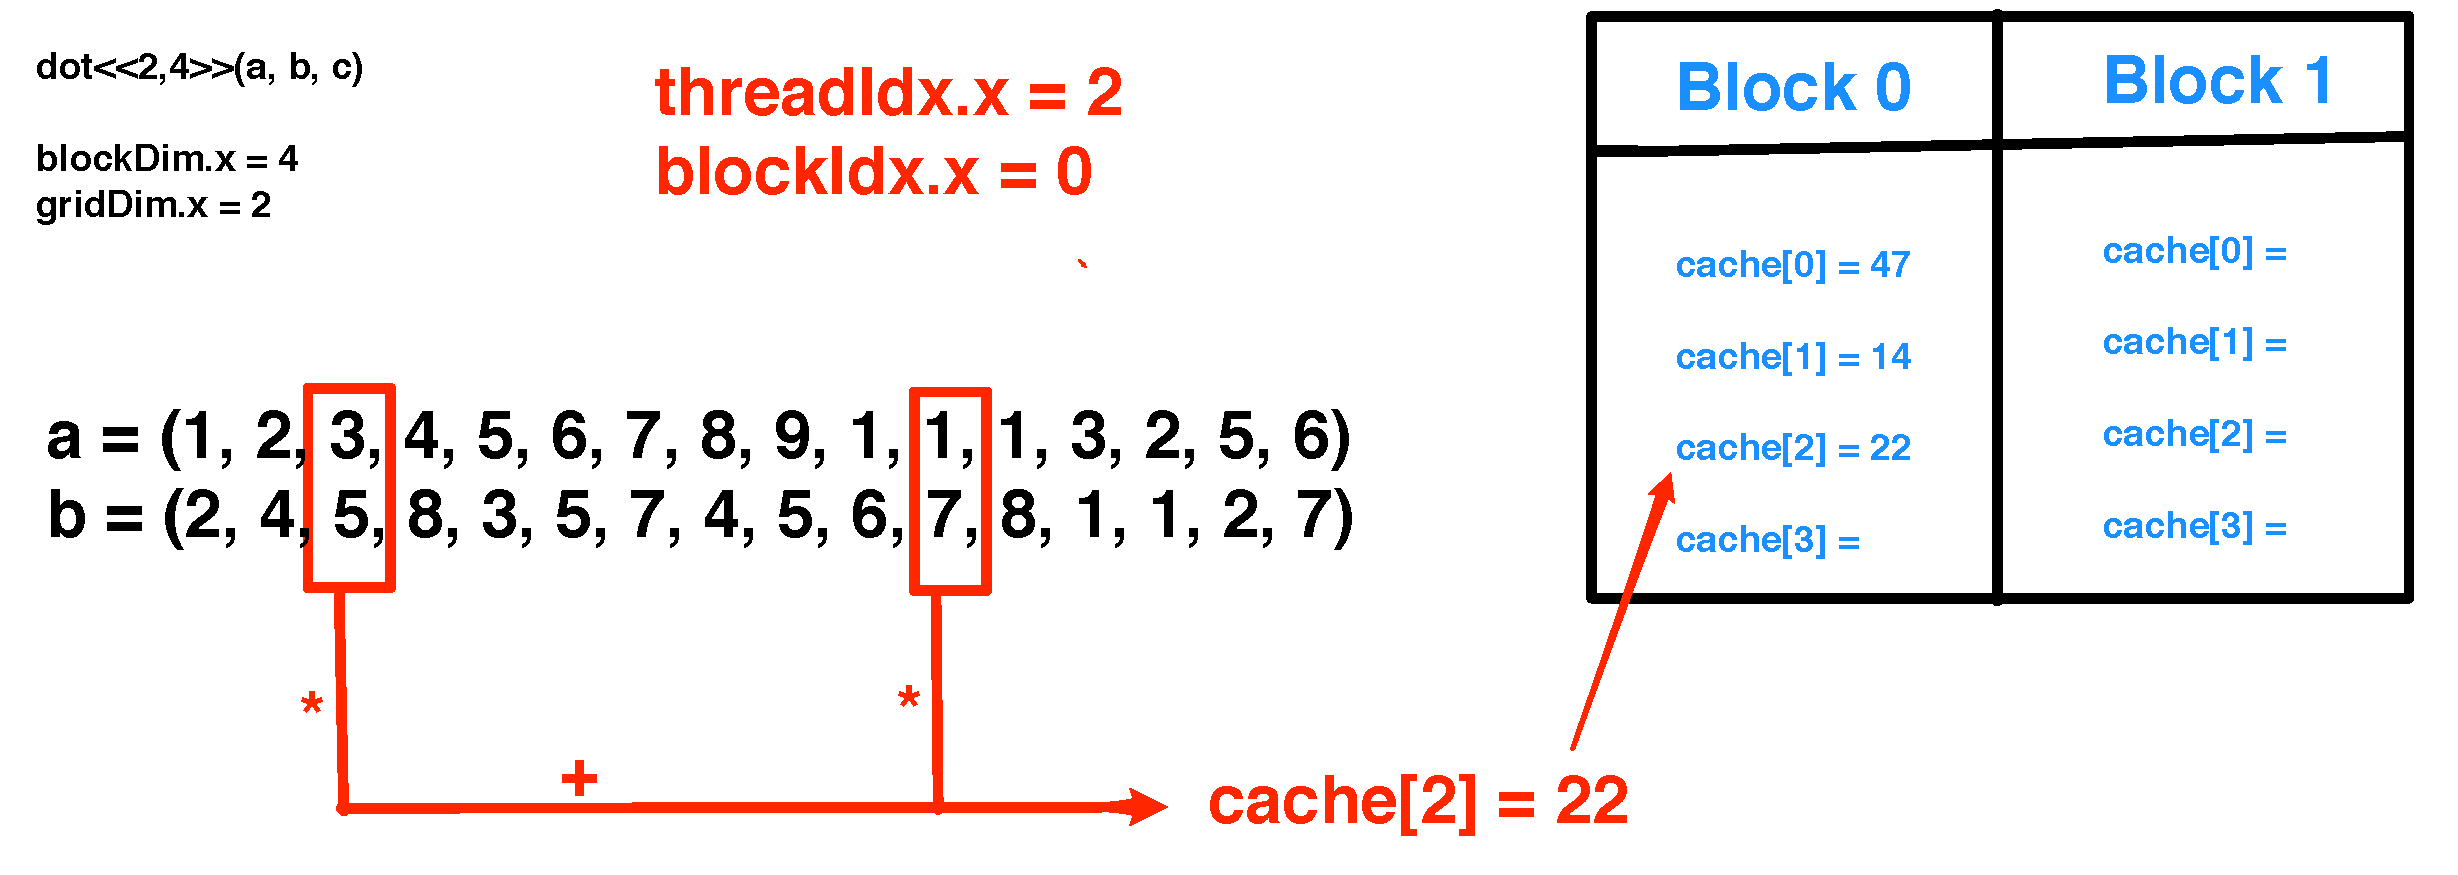
\includegraphics[scale=.23]{../../fig/dotconcept4}
\end{center}
\end{frame}
 
 \begin{frame}
\frametitle{{\tt dot<<<2, 4>>>(a, b, c)} with $N = 16$}
\begin{center}
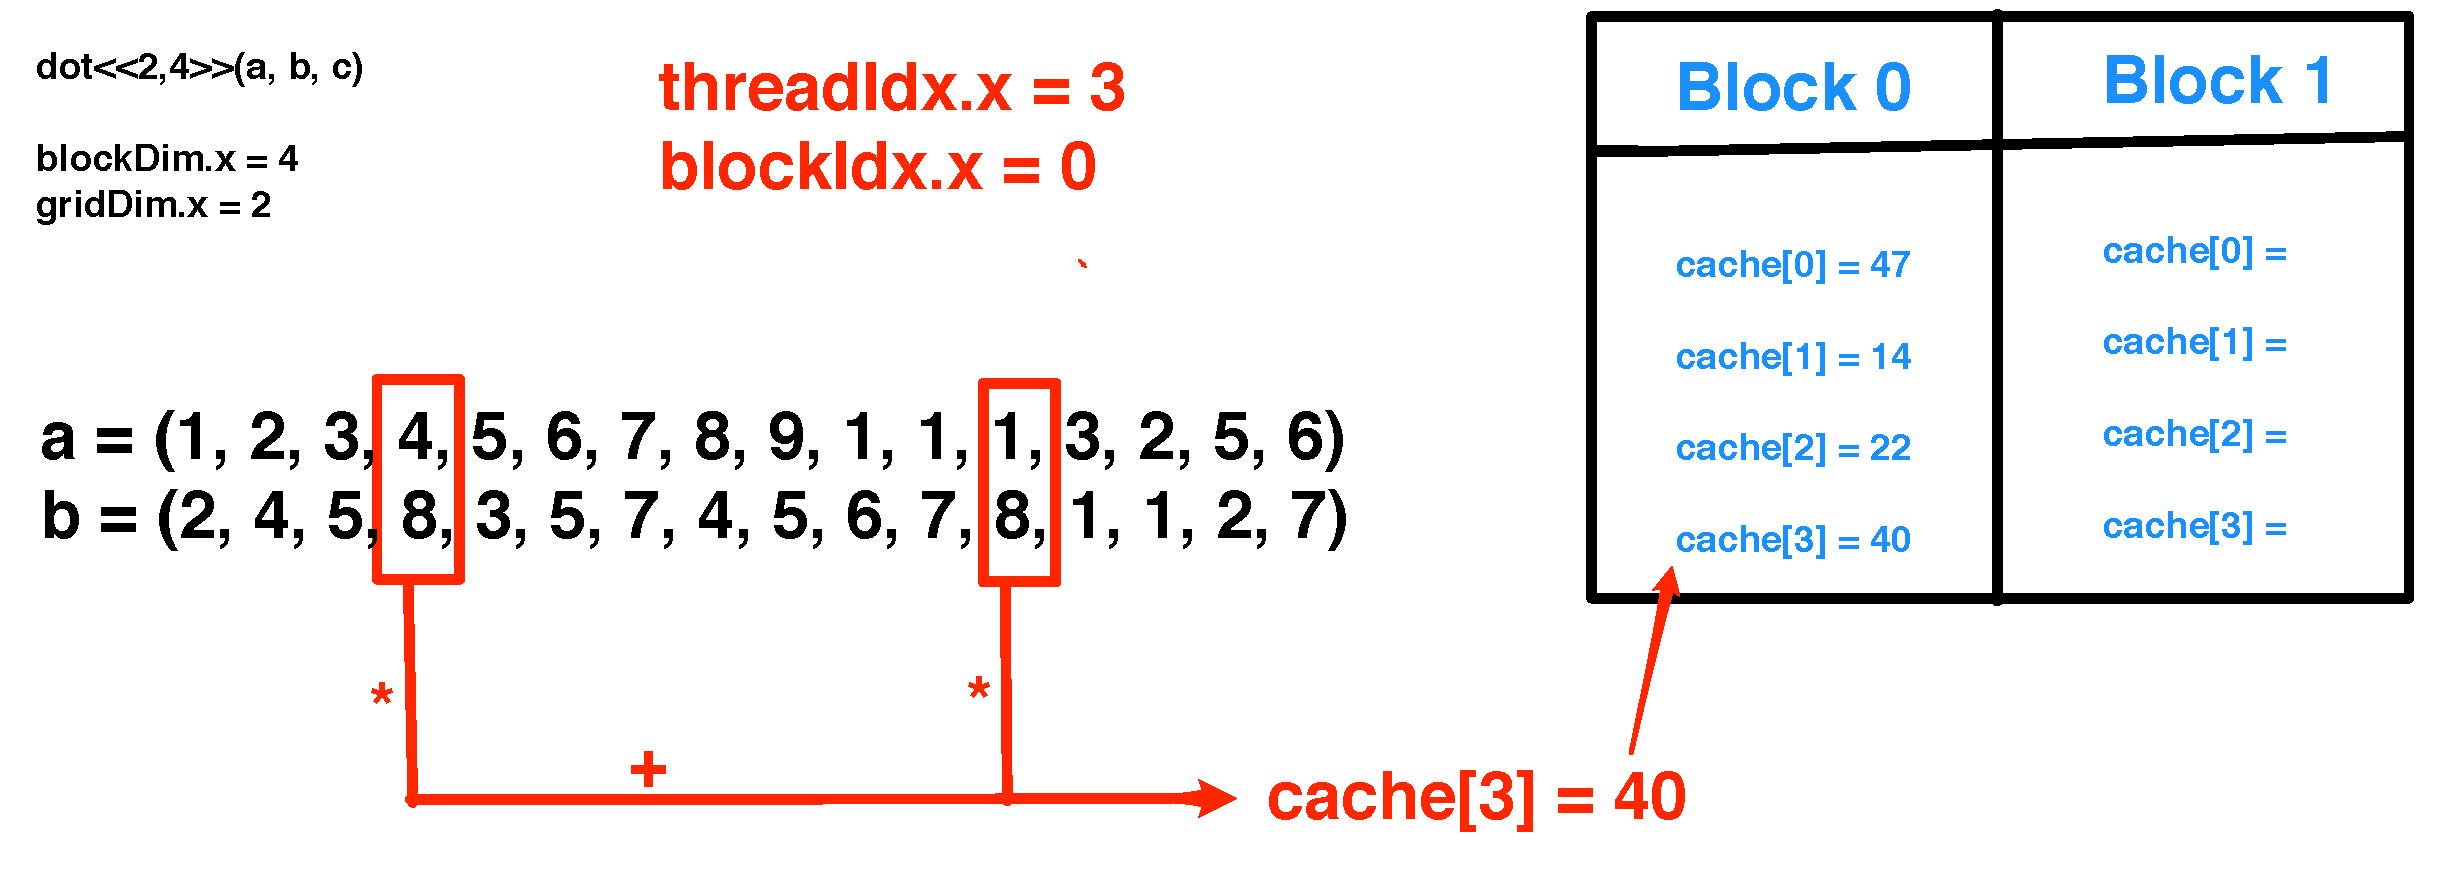
\includegraphics[scale=.23]{../../fig/dotconcept5}
\end{center}
\end{frame}
 
 \begin{frame}
\frametitle{{\tt dot<<<2, 4>>>(a, b, c)} with $N = 16$}
\begin{center}
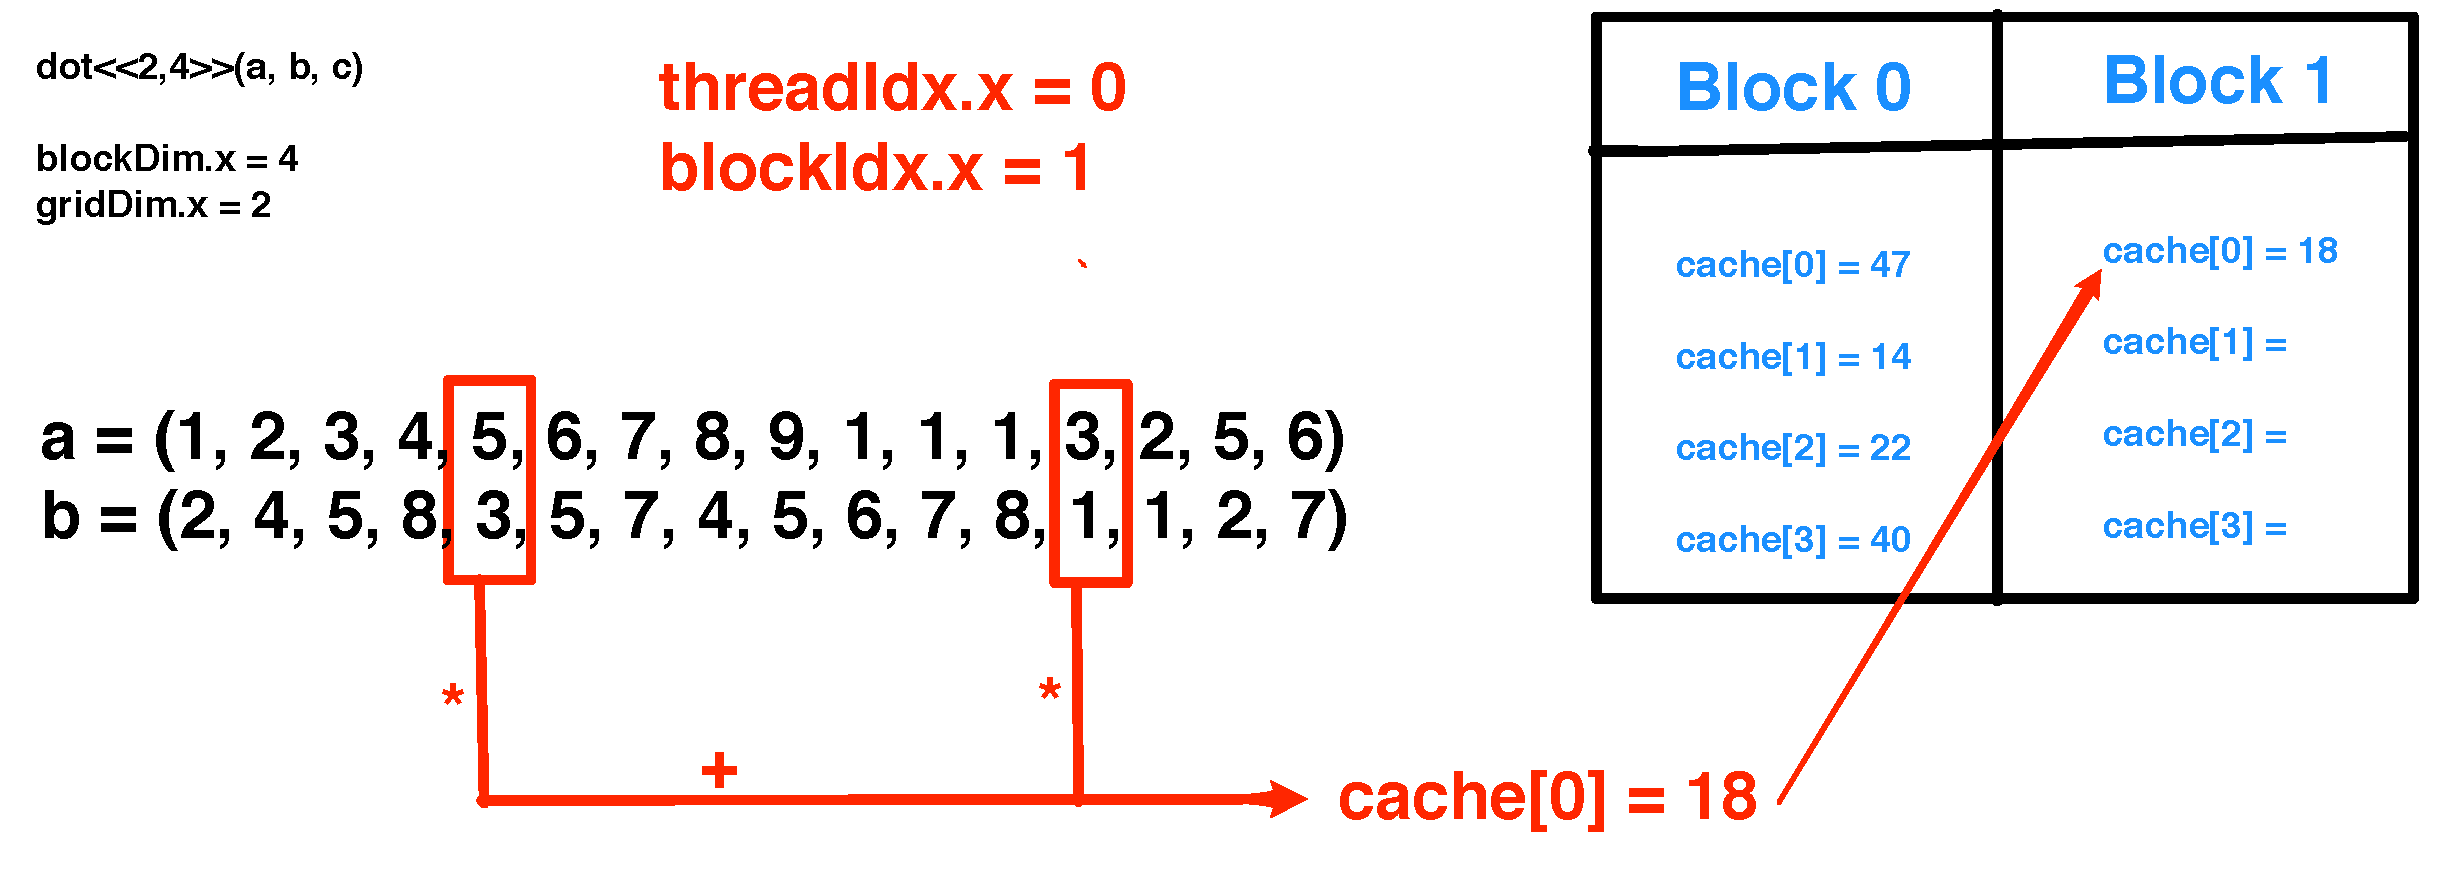
\includegraphics[scale=.23]{../../fig/dotconcept6}
\end{center}
\end{frame}
 
 \begin{frame}
\frametitle{{\tt dot<<<2, 4>>>(a, b, c)} with $N = 16$}
\begin{center}
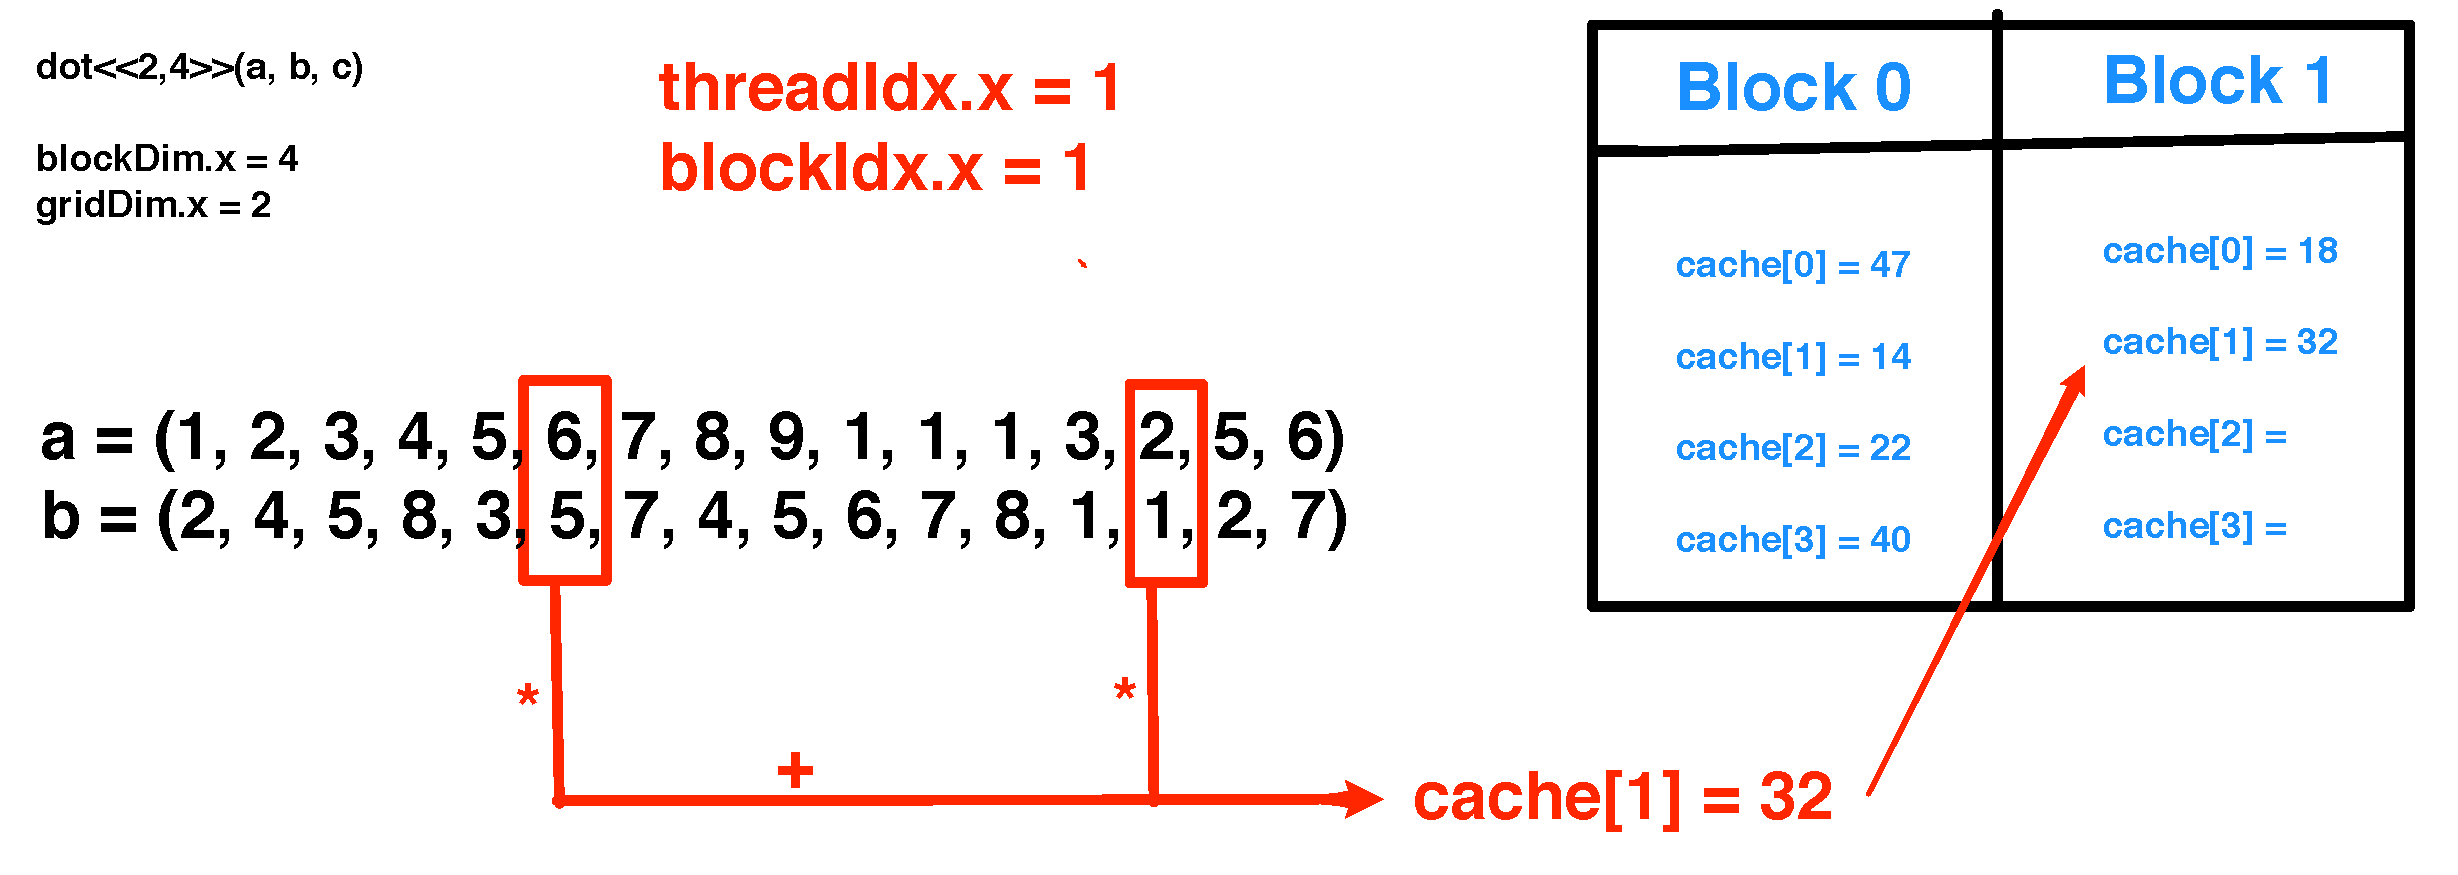
\includegraphics[scale=.23]{../../fig/dotconcept7}
\end{center}
\end{frame}
 
 \begin{frame}
\frametitle{{\tt dot<<<2, 4>>>(a, b, c)} with $N = 16$}
\begin{center}
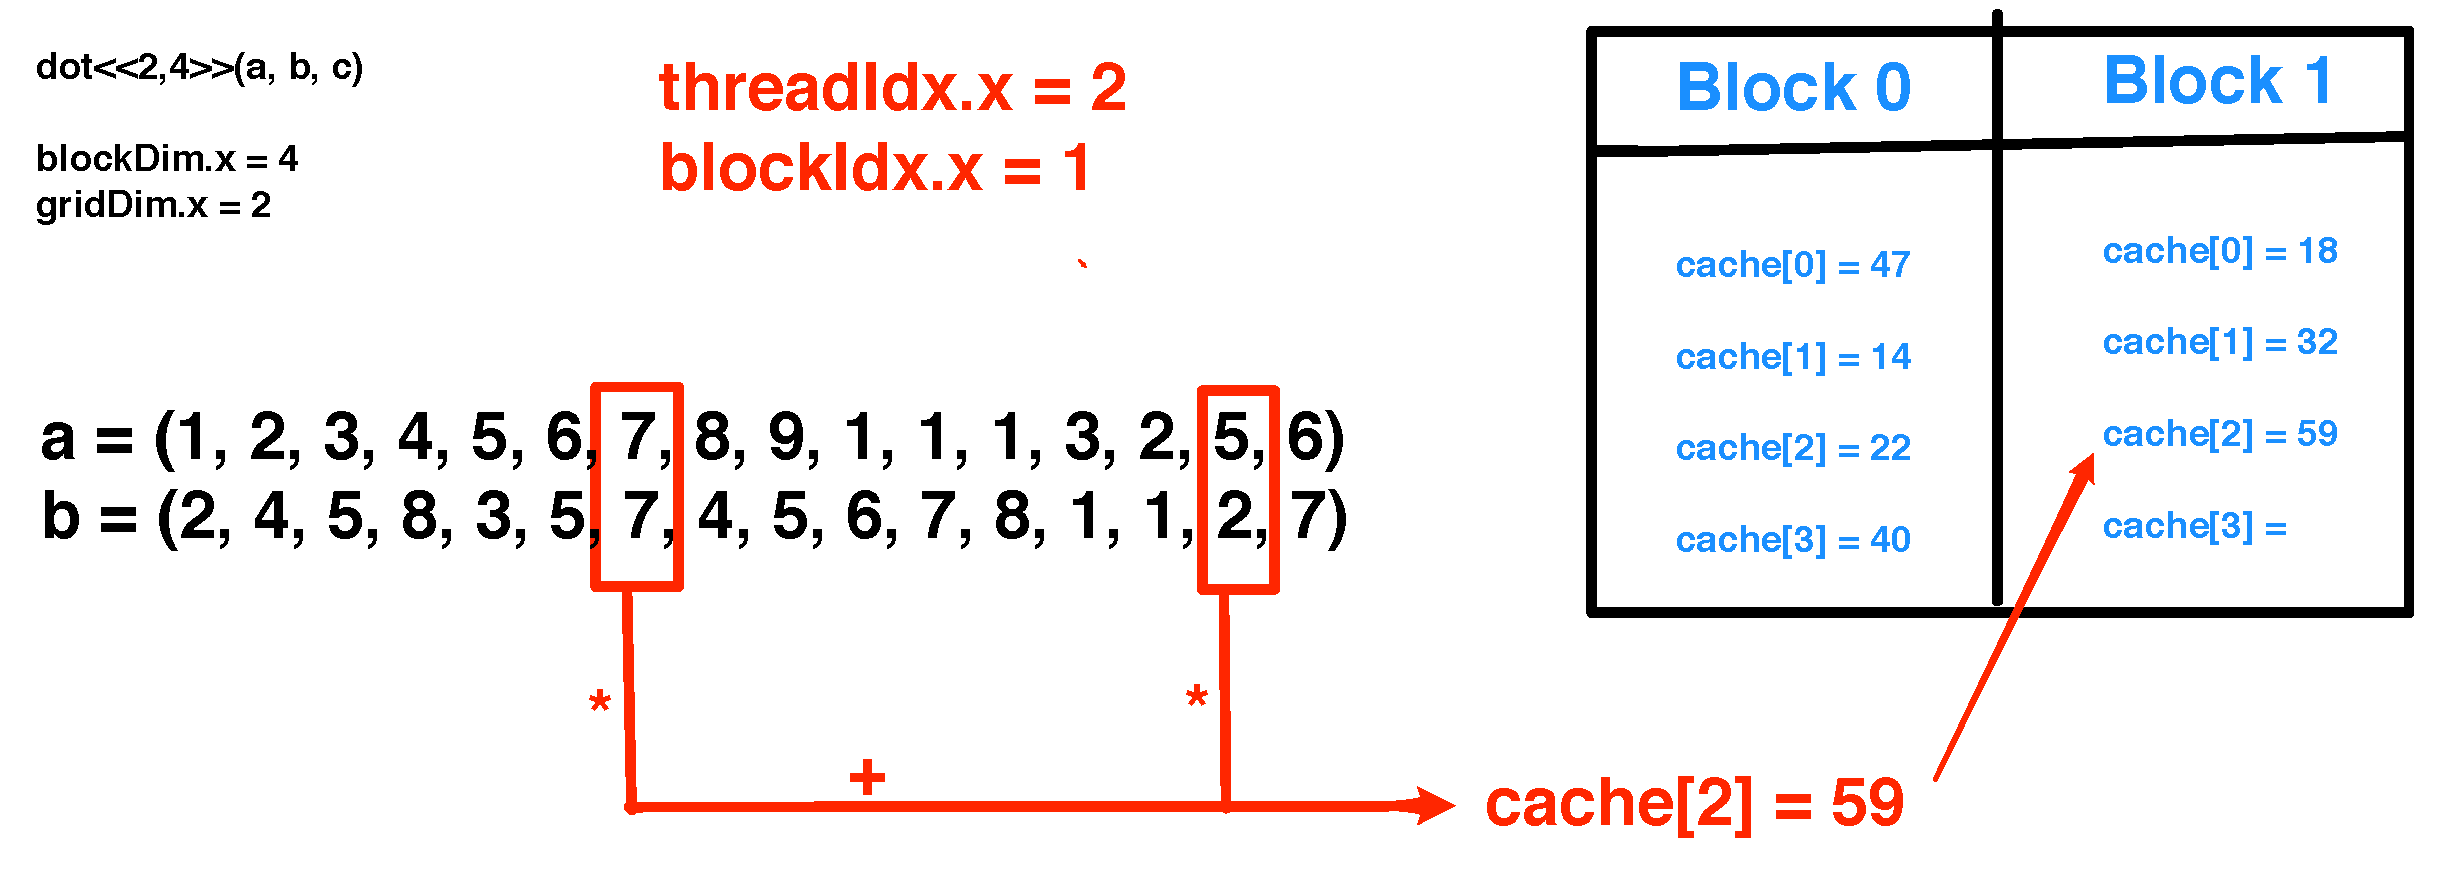
\includegraphics[scale=.23]{../../fig/dotconcept8}
\end{center}
\end{frame}
 
 \begin{frame}
\frametitle{{\tt dot<<<2, 4>>>(a, b, c)} with $N = 16$}
\begin{center}
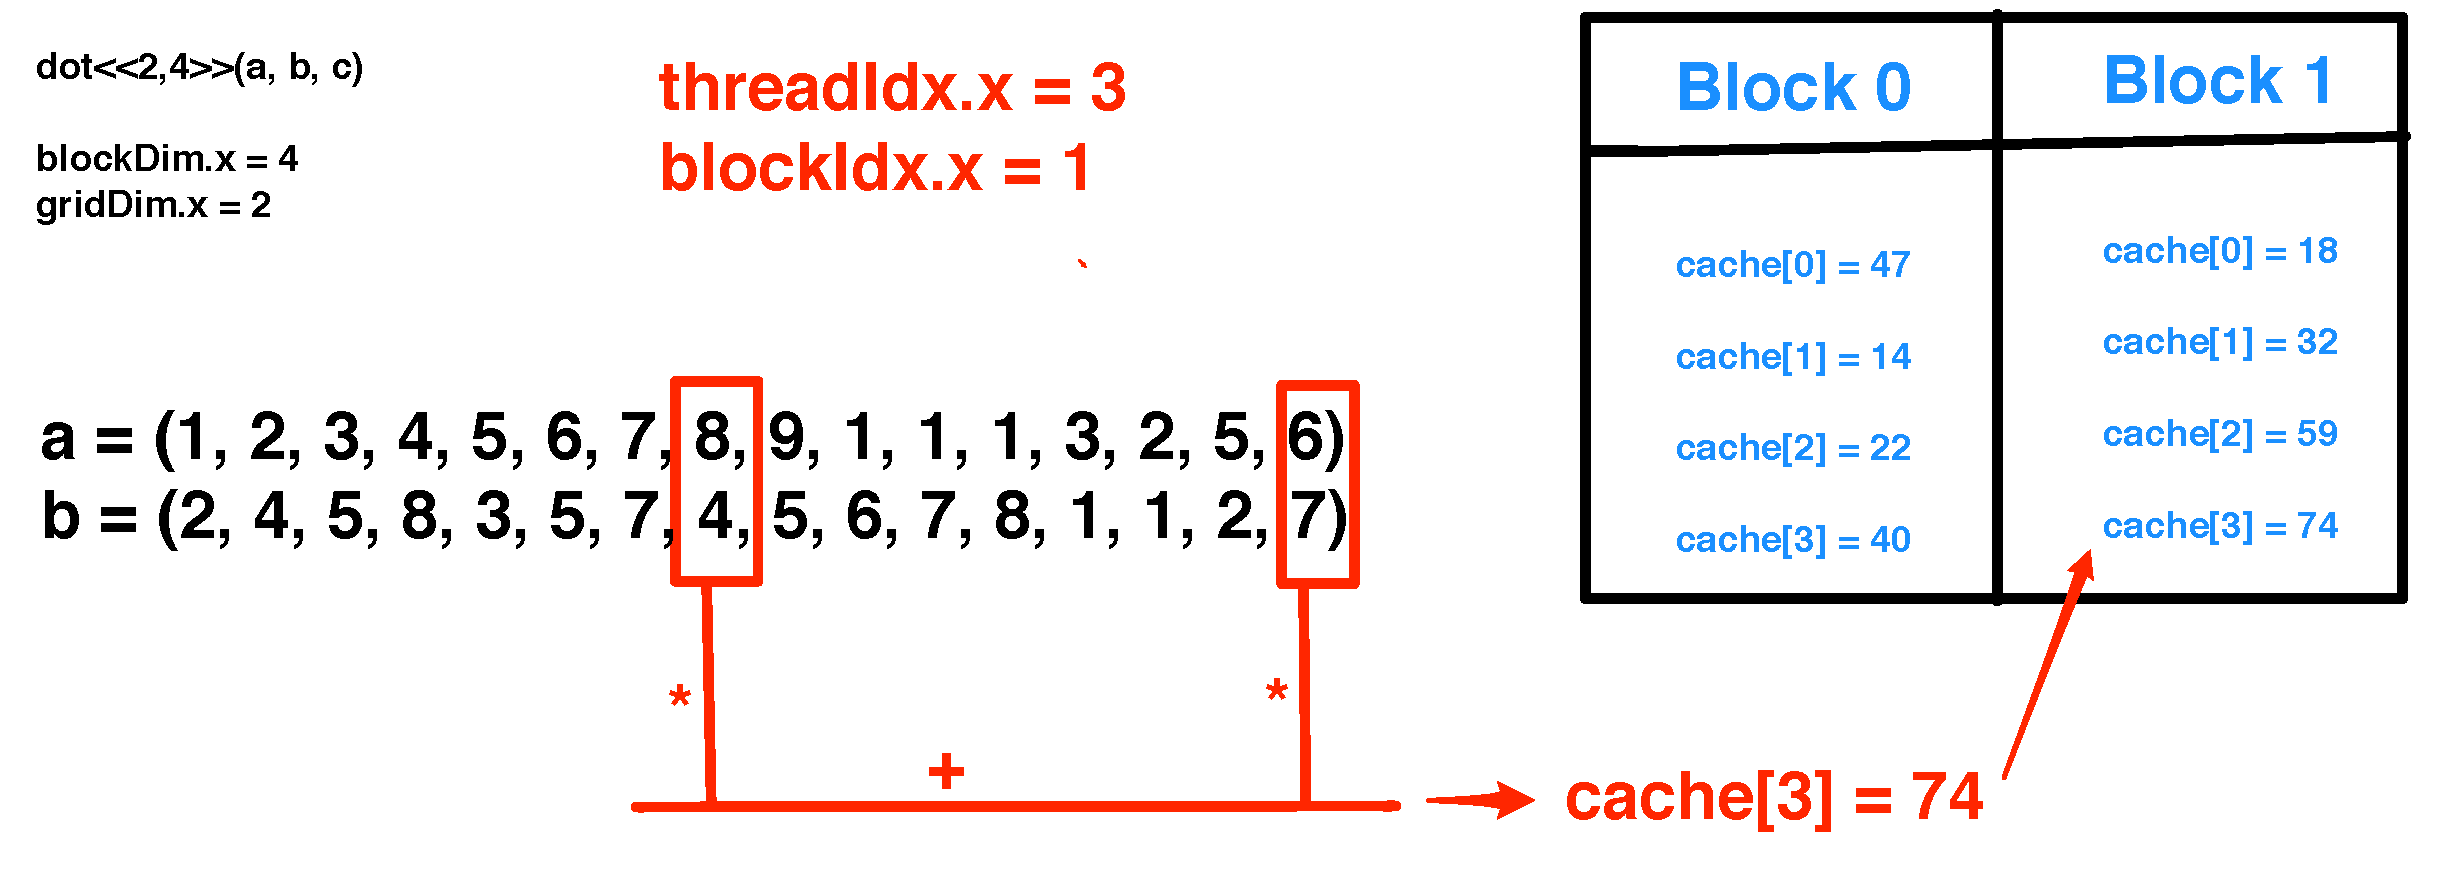
\includegraphics[scale=.23]{../../fig/dotconcept9}
\end{center}
\end{frame}
 
\begin{frame}[fragile]
\begin{itemize} \lstset{basicstyle=\tiny}
\item Make sure {\tt cache} is full before continuing.
\end{itemize}

\begin{lstlisting}[name=dp]
// synchronize threads in this block
__syncthreads();
\end{lstlisting}


\begin{itemize}
\pause \item Execute a pairwise sum of {\tt cache} for each block.
\end{itemize}

\begin{lstlisting}[name=dp]
  // threadsPerBlock must be a power of 2 
  int i = blockDim.x/2;
  while (i != 0) {
    if (cacheIndex < i)
      cache[cacheIndex] += cache[cacheIndex + i];
    __syncthreads();   
    i /= 2; 
  }
\end{lstlisting}

\begin{itemize}
\pause \item Record the result in {\tt partial\_c}.
\end{itemize}

\begin{lstlisting}[name=dp]
  if (cacheIndex == 0) 
    partial_c[blockIdx.x] = cache[0];
}
\end{lstlisting}
\end{frame}

\begin{frame}
\frametitle{{\tt dot<<<2, 4>>>(a, b, c)} with $N = 16$}
\begin{center}
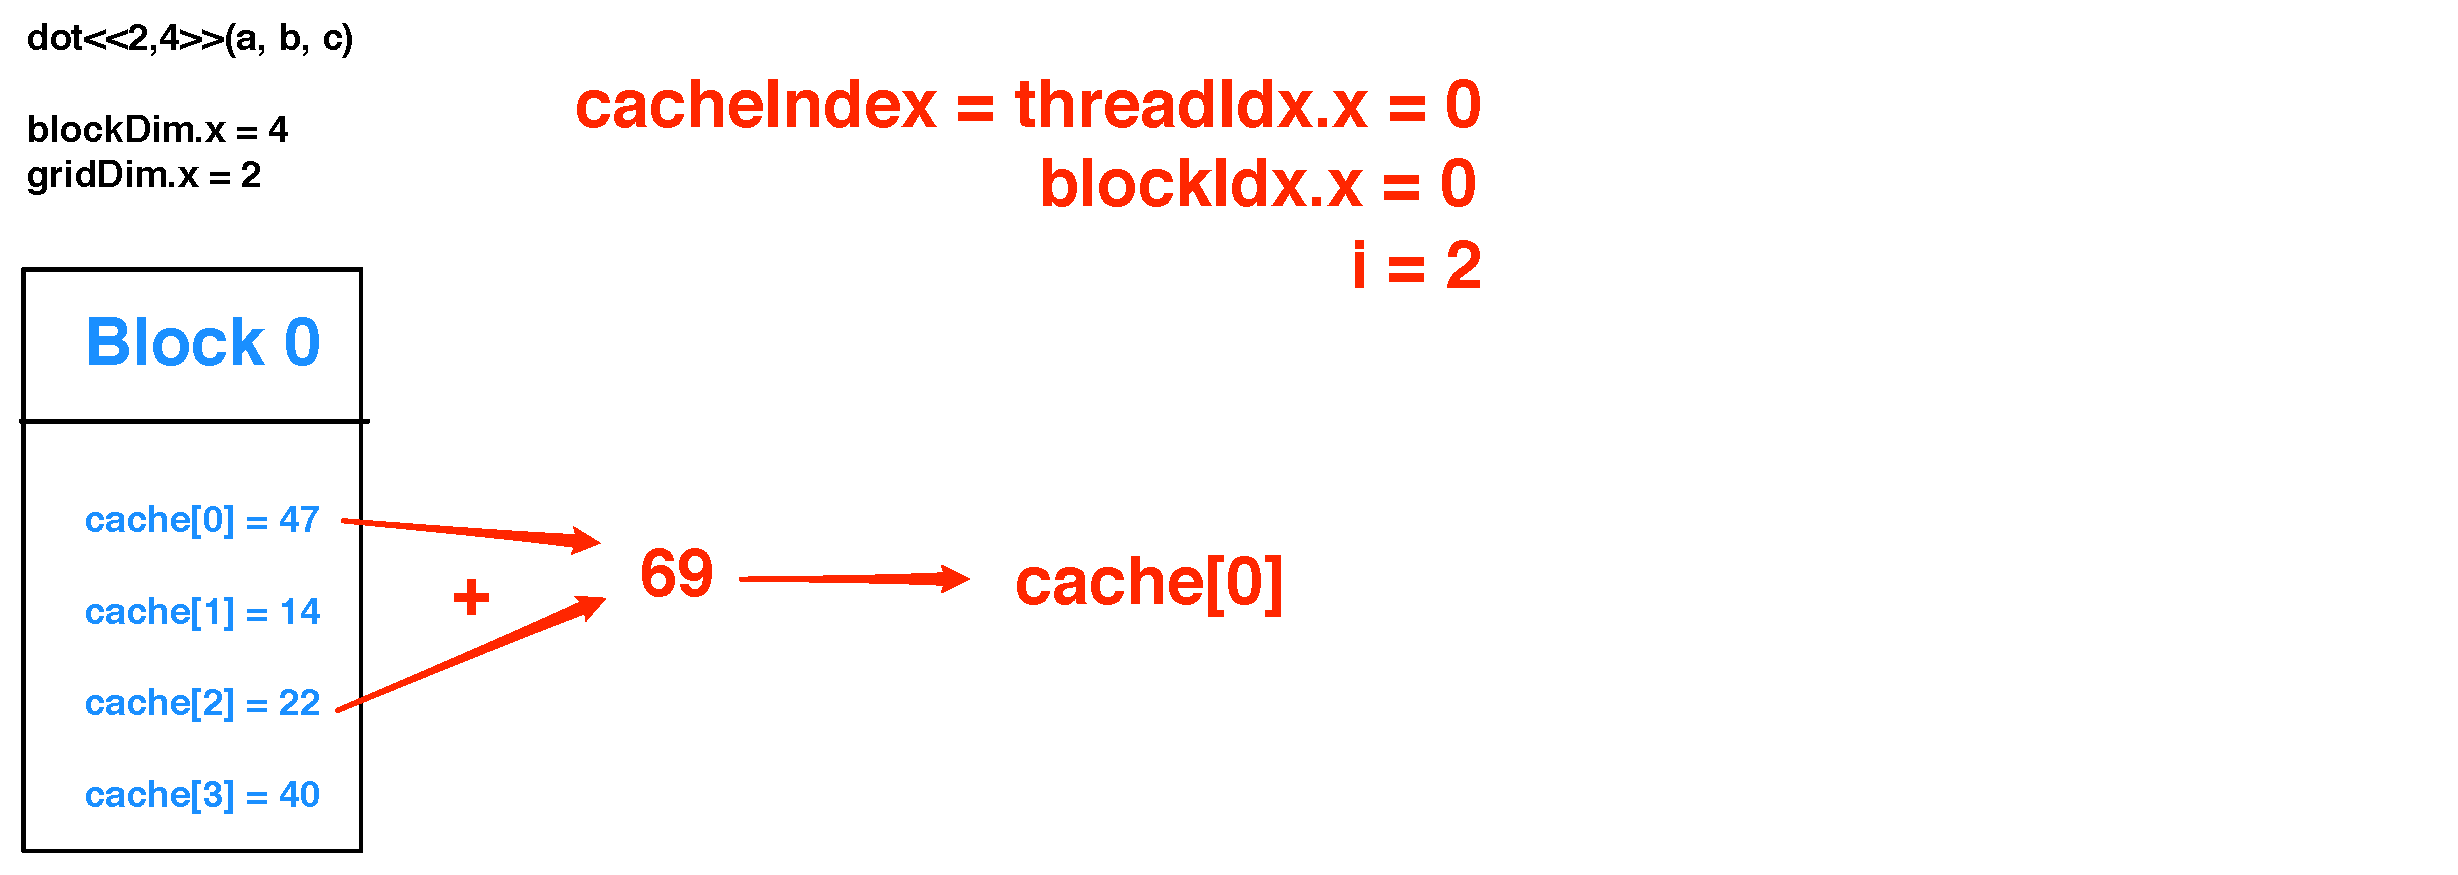
\includegraphics[scale=.3]{../../fig/dotconcept10}
\end{center}
\end{frame}

\begin{frame}
\frametitle{{\tt dot<<<2, 4>>>(a, b, c)} with $N = 16$}
\begin{center}
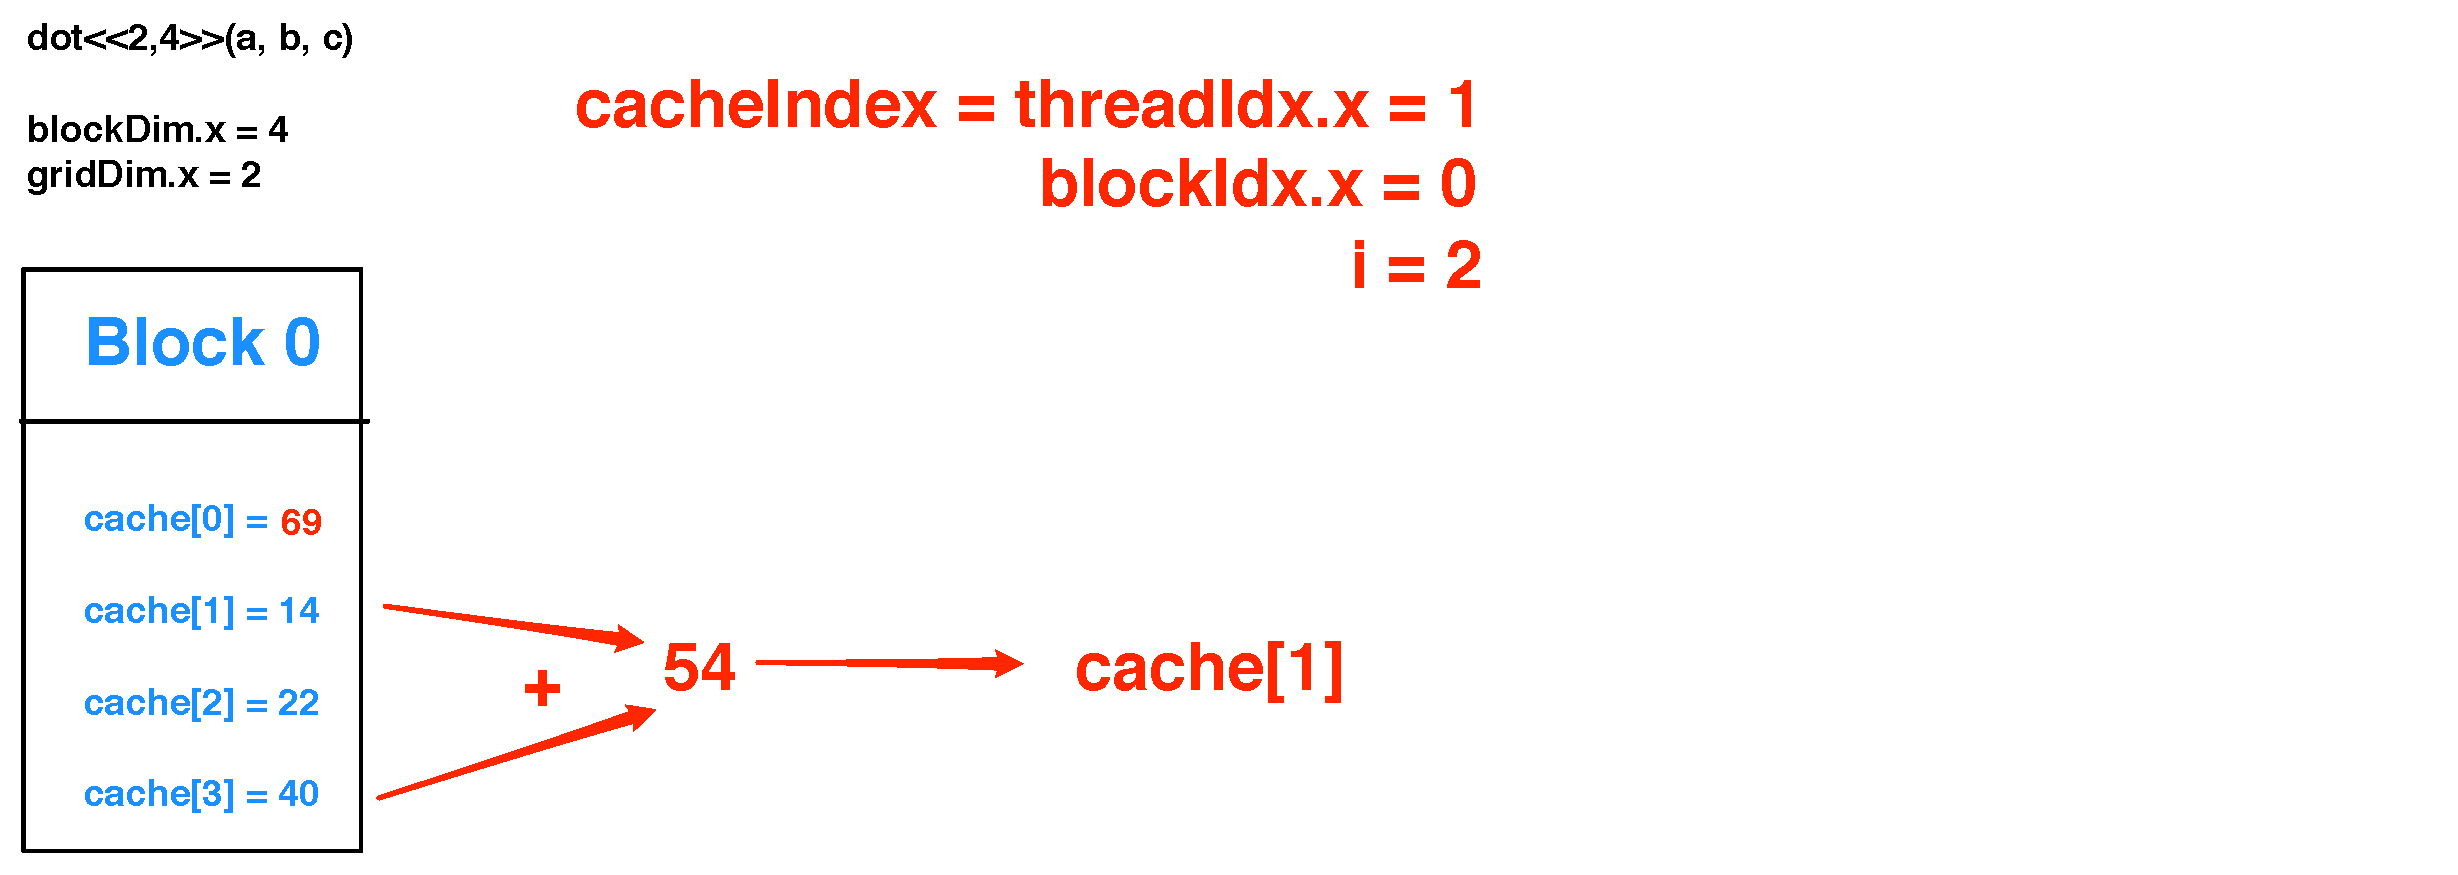
\includegraphics[scale=.3]{../../fig/dotconcept11}
\end{center}
\end{frame}

\begin{frame}
\frametitle{{\tt dot<<<2, 4>>>(a, b, c)} with $N = 16$}
\begin{center}
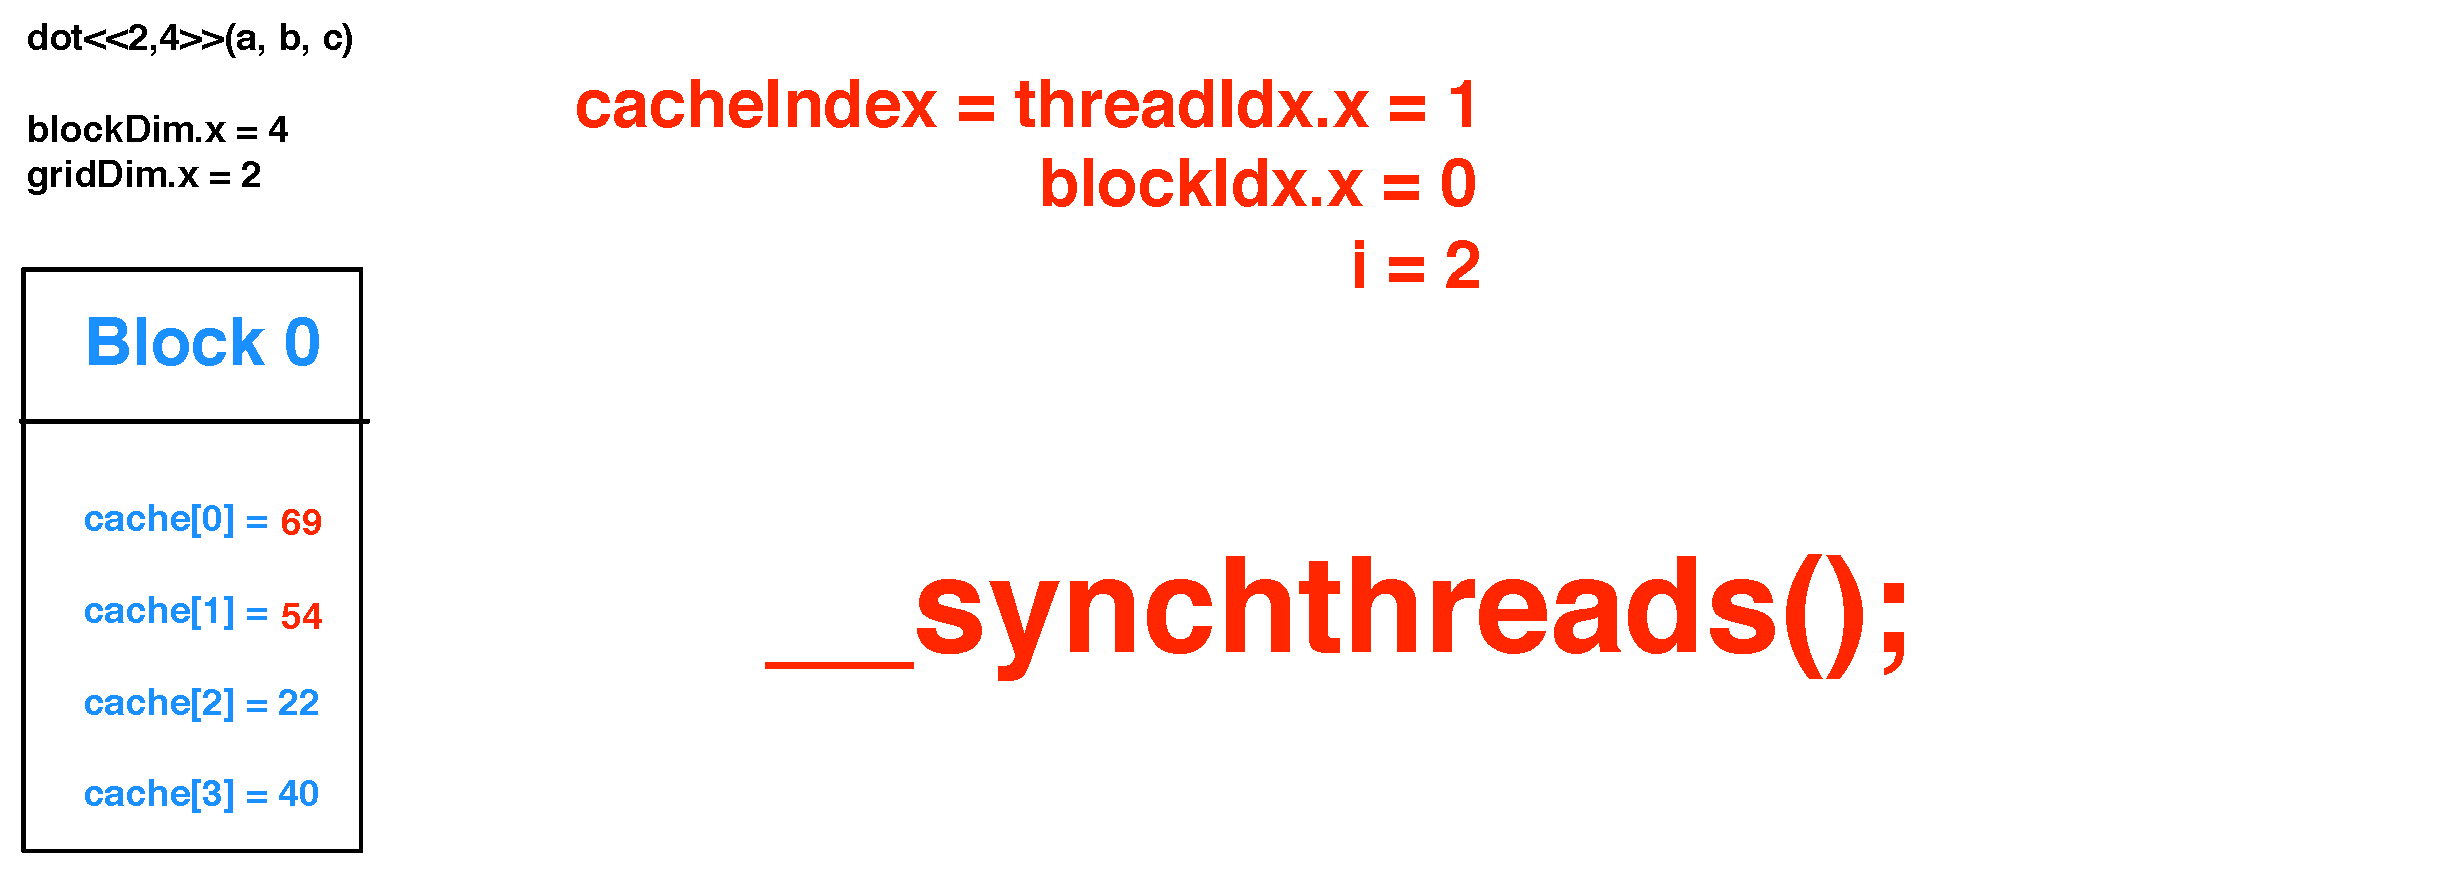
\includegraphics[scale=.3]{../../fig/dotconcept12}
\end{center}
\end{frame}

\begin{frame}
\frametitle{{\tt dot<<<2, 4>>>(a, b, c)} with $N = 16$}
\begin{center}
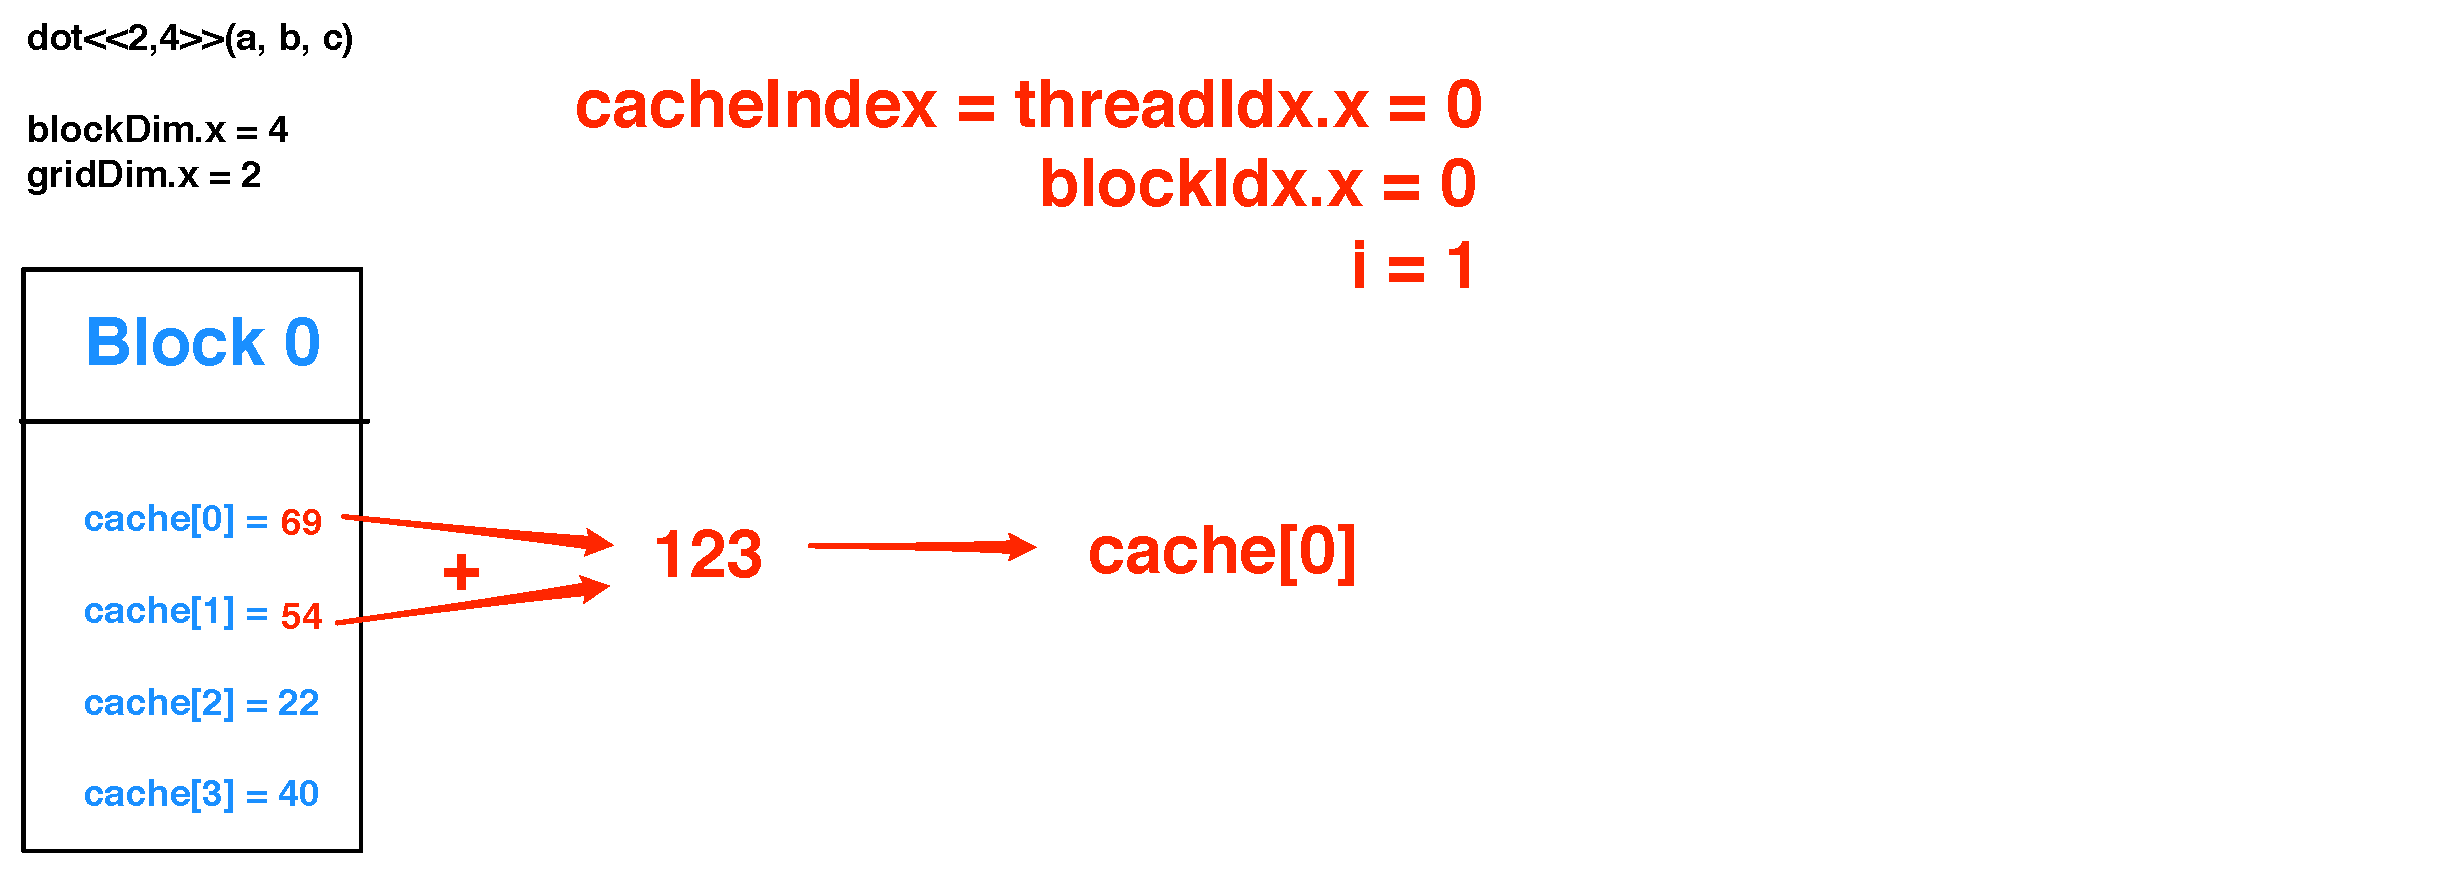
\includegraphics[scale=.3]{../../fig/dotconcept13}
\end{center}
\end{frame}

\begin{frame}
\frametitle{{\tt dot<<<2, 4>>>(a, b, c)} with $N = 16$}
\begin{center}
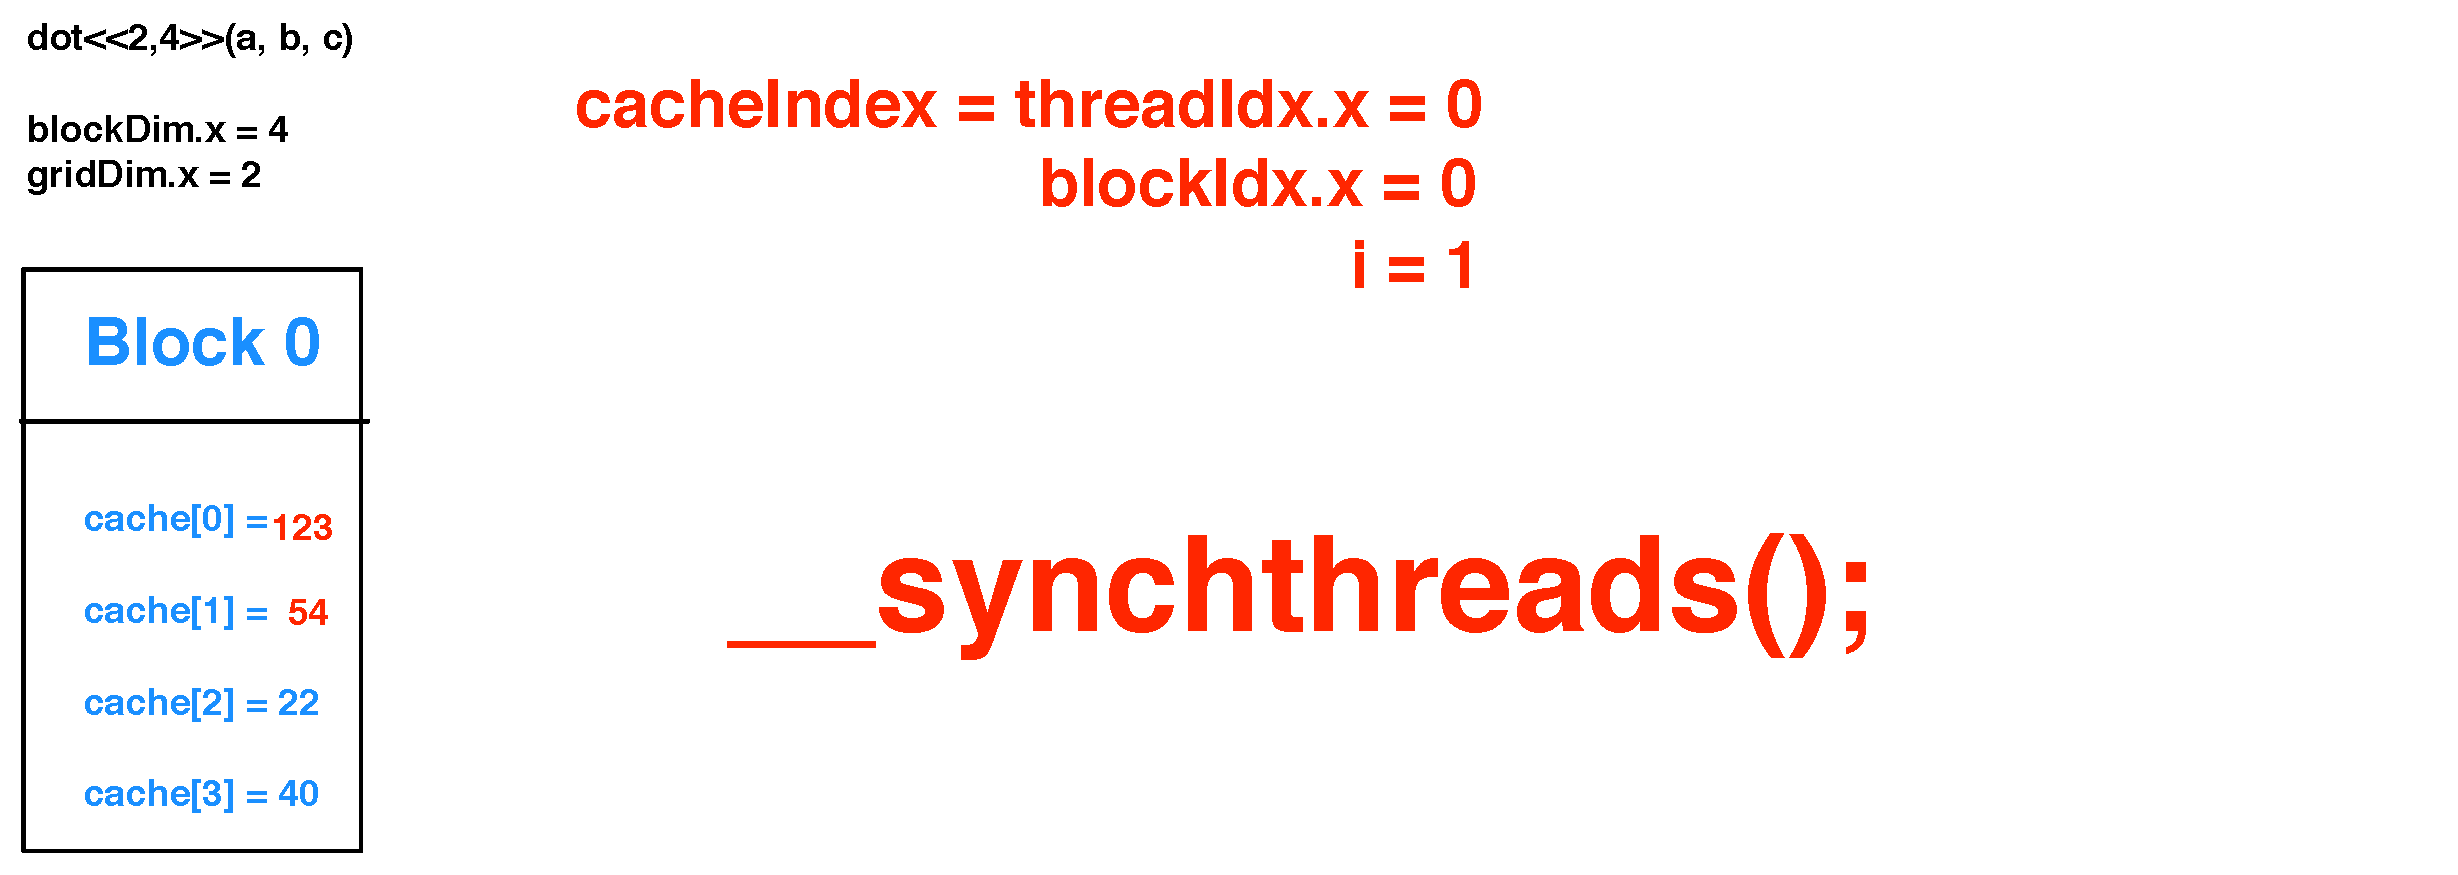
\includegraphics[scale=.3]{../../fig/dotconcept14}
\end{center}
\end{frame}

\begin{frame}
\frametitle{{\tt dot<<<2, 4>>>(a, b, c)} with $N = 16$}
\begin{center}
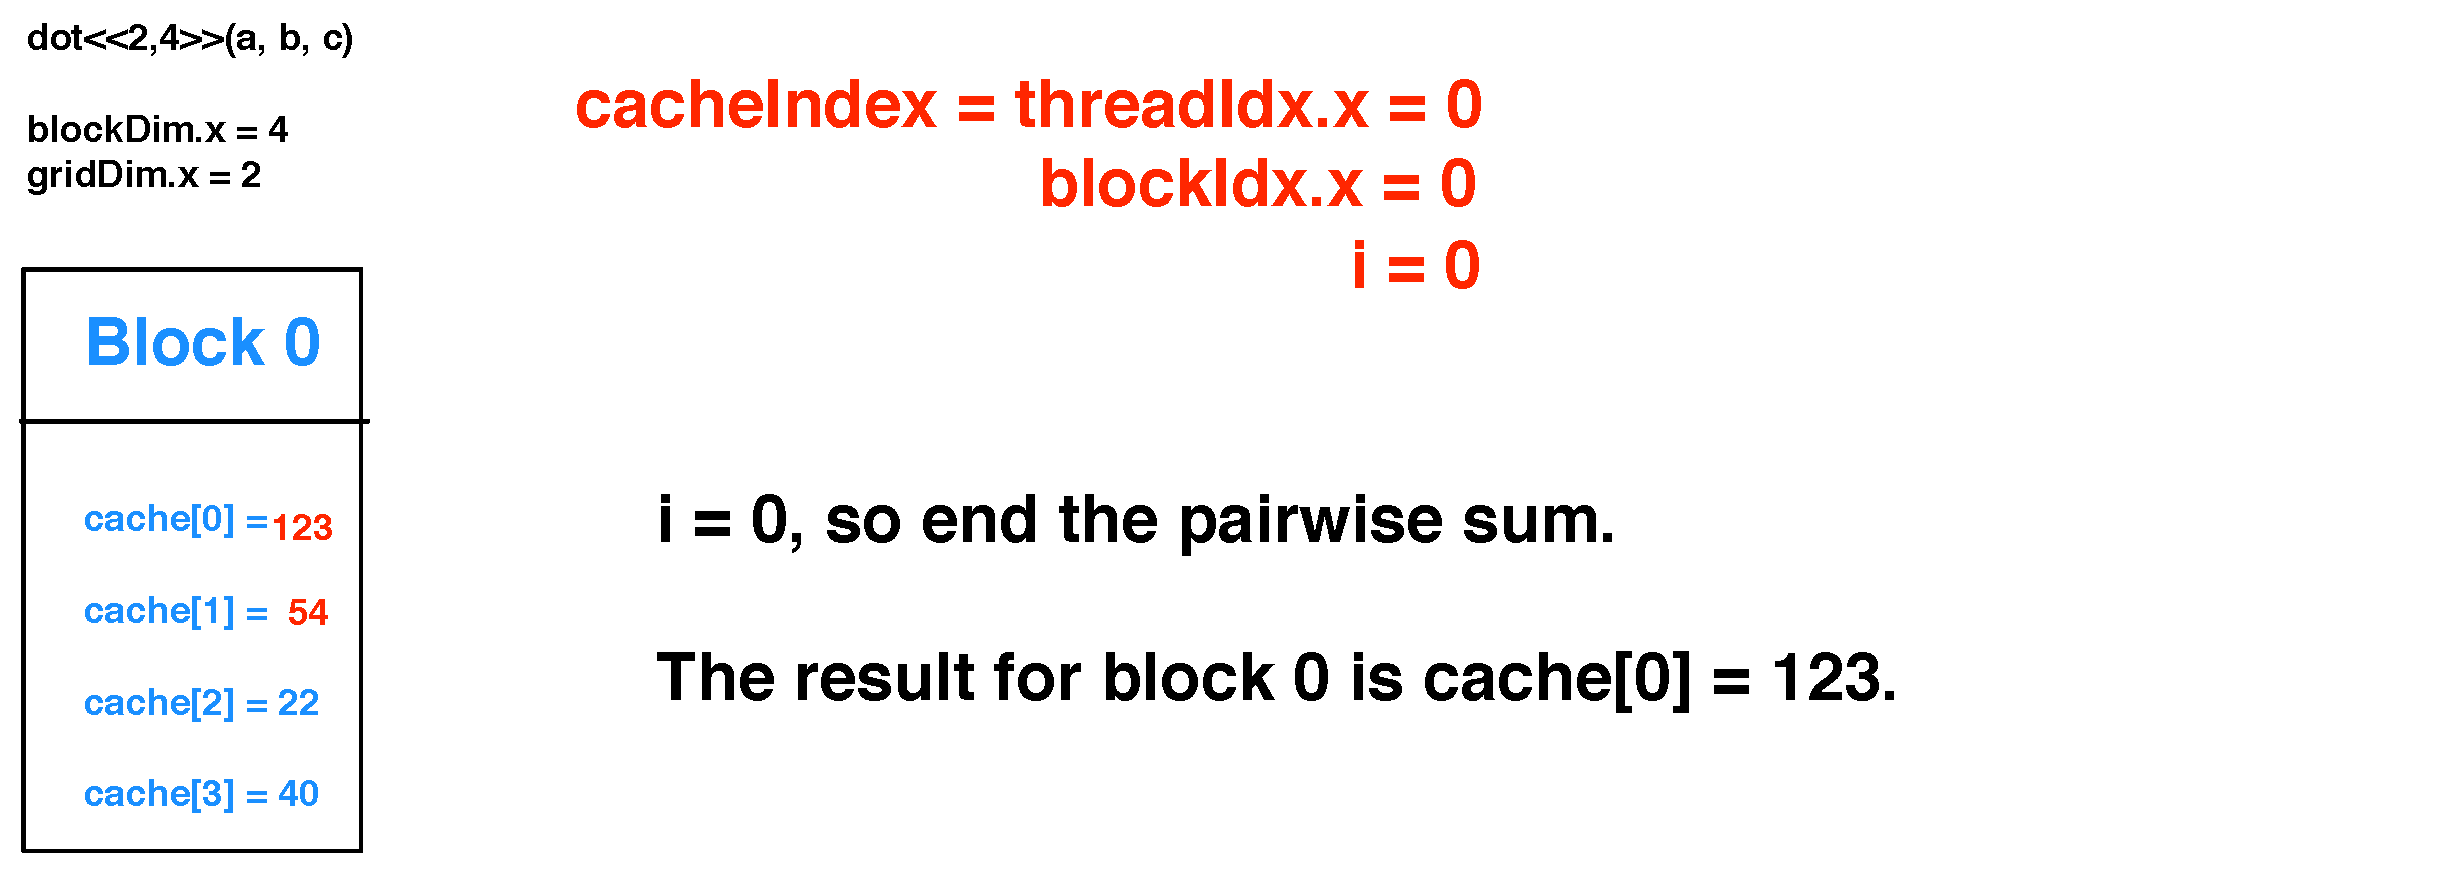
\includegraphics[scale=.3]{../../fig/dotconcept15}
\end{center}
\end{frame}

\begin{frame}[fragile]
\frametitle{Sum up {\tt partial\_c} inside {\tt int main()}}

\begin{lstlisting}[name=dp]
  dot<<<blocksPerGrid,threadsPerBlock>>>( dev_a, dev_b, dev_partial_c );   

  // copy partial_c to the CPU
  cudaMemcpy(partial_c, dev_partial_c, blocksPerGrid*sizeof(float), cudaMemcpyDeviceToHost);

  // finish up on the CPU side
  c = 0;
  for (int i=0; i<blocksPerGrid; i++) {
    c += partial_c[i];
  }
\end{lstlisting}
\end{frame}


\begin{frame}
\frametitle{Outline}
\tableofcontents
\end{frame}

\begin{frame}
\frametitle{Resources} \small

\begin{itemize}
\item Guides:
\begin{enumerate}
 \item J. Sanders and E. Kandrot. {CUDA by Example.} Addison-Wesley, 2010.
\pause \item D. Kirk, W.H. Wen-mei, and W. Hwu. \emph{Programming massively parallel processors: a hands-on approach.} Morgan Kaufmann, 2010.
\pause \item Michael Romero and Rodrigo Urra. �CUDA Programming.� Rochester Institute of Technology. \url{http://cuda.ce.rit.edu/cuda overview/cuda overview.html}.
\end{enumerate}
\pause \item Code:
\begin{itemize}
\item \href{http://will-landau.com/gpu/Code/CUDA_C/time/time.cu}{time.cu}
\item \href{http://will-landau.com/gpu/Code/CUDA_C/pairwise_sum_timed/pairwise_sum_timed.cu}{pairwise\_sum\_timed.cu}
\item \href{http://will-landau.com/gpu/Code/CUDA_C/dot_product/dot_product.cu}{dot\_product.cu}
\end{itemize}
\end{itemize}
\end{frame}


\begin{frame}
\frametitle{That's all for today.}
\begin{itemize}
\item Series materials are available at \url{http://will-landau.com/gpu}.
\end{itemize}
\end{frame}


\end{document}